% Options for packages loaded elsewhere
\PassOptionsToPackage{unicode}{hyperref}
\PassOptionsToPackage{hyphens}{url}
\PassOptionsToPackage{dvipsnames,svgnames,x11names}{xcolor}
%
\documentclass[
  10pt,
]{article}
\usepackage{amsmath,amssymb}
\usepackage{iftex}
\ifPDFTeX
  \usepackage[T1]{fontenc}
  \usepackage[utf8]{inputenc}
  \usepackage{textcomp} % provide euro and other symbols
\else % if luatex or xetex
  \usepackage{unicode-math} % this also loads fontspec
  \defaultfontfeatures{Scale=MatchLowercase}
  \defaultfontfeatures[\rmfamily]{Ligatures=TeX,Scale=1}
\fi
\usepackage{lmodern}
\ifPDFTeX\else
  % xetex/luatex font selection
  \setmainfont[]{DejaVu Serif}
  \setsansfont[]{DejaVu Sans}
  \setmonofont[]{DejaVu Sans Mono}
  \setmathfont[]{Latin Modern Math}
\fi
% Use upquote if available, for straight quotes in verbatim environments
\IfFileExists{upquote.sty}{\usepackage{upquote}}{}
\IfFileExists{microtype.sty}{% use microtype if available
  \usepackage[]{microtype}
  \UseMicrotypeSet[protrusion]{basicmath} % disable protrusion for tt fonts
}{}
\makeatletter
\@ifundefined{KOMAClassName}{% if non-KOMA class
  \IfFileExists{parskip.sty}{%
    \usepackage{parskip}
  }{% else
    \setlength{\parindent}{0pt}
    \setlength{\parskip}{6pt plus 2pt minus 1pt}}
}{% if KOMA class
  \KOMAoptions{parskip=half}}
\makeatother
\usepackage{xcolor}
\usepackage[margin=2.0cm]{geometry}
\usepackage{longtable,booktabs,array}
\usepackage{calc} % for calculating minipage widths
% Correct order of tables after \paragraph or \subparagraph
\usepackage{etoolbox}
\makeatletter
\patchcmd\longtable{\par}{\if@noskipsec\mbox{}\fi\par}{}{}
\makeatother
% Allow footnotes in longtable head/foot
\IfFileExists{footnotehyper.sty}{\usepackage{footnotehyper}}{\usepackage{footnote}}
\makesavenoteenv{longtable}
\usepackage{graphicx}
\makeatletter
\def\maxwidth{\ifdim\Gin@nat@width>\linewidth\linewidth\else\Gin@nat@width\fi}
\def\maxheight{\ifdim\Gin@nat@height>\textheight\textheight\else\Gin@nat@height\fi}
\makeatother
% Scale images if necessary, so that they will not overflow the page
% margins by default, and it is still possible to overwrite the defaults
% using explicit options in \includegraphics[width, height, ...]{}
\setkeys{Gin}{width=\maxwidth,height=\maxheight,keepaspectratio}
% Set default figure placement to htbp
\makeatletter
\def\fps@figure{htbp}
\makeatother
\setlength{\emergencystretch}{3em} % prevent overfull lines
\providecommand{\tightlist}{%
  \setlength{\itemsep}{0pt}\setlength{\parskip}{0pt}}
\setcounter{secnumdepth}{-\maxdimen} % remove section numbering
% doc_header.tex -- LaTeX preamble additions used by build_docs.sh for every
% Markdown -> LaTeX -> PDF conversion (supplements, README, submission files).
\usepackage{etoolbox}
% longtable may not be loaded by pandoc when a document has no table
\usepackage{longtable}
% bold vectors: \bm -> \symbf under unicode-math (XeLaTeX), bm package otherwise
\makeatletter
\@ifpackageloaded{unicode-math}{\providecommand{\bm}[1]{\symbf{#1}}}{\usepackage{bm}}
\makeatother
% smaller type in long tables so that wide audit tables fit the text width;
% inside a table a line break is allowed after an underscore of plain text
% (pandoc writes it as \_), so that long identifiers wrap inside their column
% rows are set a little apart, so that symbols with indices do not touch
\AtBeginEnvironment{longtable}{\footnotesize\renewcommand{\arraystretch}{1.45}%
  \let\sptunderscore\_\def\_{\sptunderscore\allowbreak}}
\setlength{\LTcapwidth}{\textwidth}
% allow line breaks after slashes and hyphens inside table cells
\usepackage{xurl}
% code blocks: break over-long lines instead of running into the margin.
% Plain ``` blocks are typeset by pandoc as {verbatim}, highlighted ones
% (```bash) as {Highlighting}; both are re-declared as breakable fancyvrb
% environments.  The continuation line is marked with a small hooked arrow.
\usepackage{fvextra}
\RecustomVerbatimEnvironment{verbatim}{Verbatim}{breaklines,breakanywhere,fontsize=\small}
\makeatletter
\@ifundefined{Highlighting}{}{%
  \RecustomVerbatimEnvironment{Highlighting}{Verbatim}{breaklines,breakanywhere,fontsize=\small,commandchars=\\\{\}}}
\makeatother
% inline code (pandoc writes it as \texttt{...}): never hyphenate -- an inserted
% hyphen could be read as part of a file name -- but allow a line break after
% an underscore, slash, comma, colon or equals sign, so that long paths and
% column lists wrap inside the text width and inside table columns.
% Inside a formula (e.g. the name of a notebook symbol in an equation) the same
% command must first leave math mode, which \text of amsmath does.
\ExplSyntaxOn
\tl_new:N \l__spt_code_tl
\cs_new_protected:Npn \__spt_texttt:n #1
  {
    \tl_set:Nn \l__spt_code_tl {#1}
    \regex_replace_all:nnN { ([\/\,\:\=]) } { \1 \c{allowbreak} } \l__spt_code_tl
    \regex_replace_all:nnN { \c{_} } { \c{_} \c{allowbreak} } \l__spt_code_tl
    \group_begin: \ttfamily \hyphenchar \font = -1 \scan_stop: \l__spt_code_tl \group_end:
  }
\RenewDocumentCommand \texttt { m }
  {
    \mode_if_math:TF { \text { \__spt_texttt:n {#1} } } { \__spt_texttt:n {#1} }
  }
\ExplSyntaxOff
% A figure is written in the Markdown source as an image paragraph followed by
% a caption paragraph ("**Figure S1.** ..."), so that the caption is also
% visible on GitHub.  An image that starts a paragraph is centered.
\usepackage{graphicx}% pandoc loads it only for documents that contain an image
\NewCommandCopy\sptincludegraphics\includegraphics
\RenewDocumentCommand\includegraphics{O{} m}{%
  \ifvmode\begin{center}\sptincludegraphics[#1]{#2}\end{center}%
  \else\sptincludegraphics[#1]{#2}\fi}
% keep figures where they are referenced
\usepackage{float}
\floatplacement{figure}{H}
% running header with the document title
\usepackage{fancyhdr}
\pagestyle{fancy}
\fancyhf{}
\fancyhead[L]{\small PROJECT spacetimes --- documentation and provenance}
\fancyhead[R]{\small\thepage}
\renewcommand{\headrulewidth}{0.4pt}
% 16x16 matrices: tighter columns so that a full matrix fits the text width
\setlength{\arraycolsep}{3.2pt}
% The documents of this project contain long tagged symbols, file paths and
% identifiers that cannot be hyphenated.  A paragraph is therefore allowed to
% have looser lines before TeX gives up and lets a line stick out of the margin.
\AtBeginDocument{\tolerance=2000 \emergencystretch=5em \hbadness=2000}
\ifLuaTeX
  \usepackage{selnolig}  % disable illegal ligatures
\fi
\IfFileExists{bookmark.sty}{\usepackage{bookmark}}{\usepackage{hyperref}}
\IfFileExists{xurl.sty}{\usepackage{xurl}}{} % add URL line breaks if available
\urlstyle{same}
\hypersetup{
  pdftitle={S4 --- The effective action for composite operators of Cornwall, Jackiw and Tomboulis, applied to the two spacetimes models},
  pdfauthor={Prepared for Patrick Lee Nash, Ph.D.},
  colorlinks=true,
  linkcolor={blue},
  filecolor={Maroon},
  citecolor={blue},
  urlcolor={blue},
  pdfcreator={LaTeX via pandoc}}

\title{S4 --- The effective action for composite operators of Cornwall,
Jackiw and Tomboulis, applied to the two spacetimes models}
\usepackage{etoolbox}
\makeatletter
\providecommand{\subtitle}[1]{% add subtitle to \maketitle
  \apptocmd{\@title}{\par {\large #1 \par}}{}{}
}
\makeatother
\subtitle{Supplement to both manuscripts of PROJECT spacetimes: the
method, independent checks of the earlier results, and what the method
predicts beyond them --- with commented source code and the provenance
of every number}
\author{Prepared for Patrick Lee Nash, Ph.D.}
\date{November 12, 2026}

\begin{document}
\maketitle

\hypertarget{purpose-and-summary-of-the-results}{%
\section{0. Purpose, and summary of the
results}\label{purpose-and-summary-of-the-results}}

The author asked that the method of J. M. Cornwall, R. Jackiw and E.
Tomboulis (Phys. Rev.~D \textbf{10}, 2428 (1974); ``CJT'' below) be
understood, be used as a check of the computations already made for the
two models, and be used to obtain every further prediction that it
gives. This supplement does the three things in that order. Section 1
explains the method for a reader who has not met it, and tests it on a
model that can be solved exactly. Section 2 writes down the CJT action
of the two models. Sections 3 to 7 apply it. Every number is produced by
the command \texttt{spacetimes\ cjt} of the Rust program (source files
\texttt{cjt\_toy.rs}, \texttt{cjt\_pairing.rs}, \texttt{cjt\_normal.rs},
\texttt{cjt\_vacuum.rs}, \texttt{cjt\_cmd.rs}, and
\texttt{symmetry.rs}); Sec. 9 says which part produces which number.

The symbols are those of ``dirac matrices'' and of Supplement S1 (cited
as S1): the fermion field of mass \(m\) with \(\nu=8\) internal states
per momentum; the Vorton-Scalar with vacuum value \(v_{VS}\), radial
mode \(s_{VS}\) of mass \(m_s\) and massless phase mode
\(\vartheta_{VS}\); the coupling \(g_{VS}=m/v_{VS}\),
\(\alpha_{VS}=g_{VS}^2/4\pi\). Unless stated otherwise the results hold
for both spacetimes, because the matrices of 7+1 and of 4+4 give the
same pairing kernels and the same internal symmetry in the sector used
(S1, Secs. 2.1 and 4.2); where the two differ, it is said.

\textbf{Checks of earlier results (all passed):}

\begin{longtable}[]{@{}
  >{\raggedright\arraybackslash}p{(\columnwidth - 4\tabcolsep) * \real{0.3404}}
  >{\raggedright\arraybackslash}p{(\columnwidth - 4\tabcolsep) * \real{0.4574}}
  >{\raggedright\arraybackslash}p{(\columnwidth - 4\tabcolsep) * \real{0.2021}}@{}}
\toprule\noalign{}
\begin{minipage}[b]{\linewidth}\raggedright
Earlier result
\end{minipage} & \begin{minipage}[b]{\linewidth}\raggedright
Check made here
\end{minipage} & \begin{minipage}[b]{\linewidth}\raggedright
Agreement
\end{minipage} \\
\midrule\noalign{}
\endhead
\bottomrule\noalign{}
\endlastfoot
gap function, fixed-point iteration (S1 Sec. 5.2) & Newton's method on
the CJT potential, different starting function &
\(1.1\times10^{-11}\) \\
gaps stored in \texttt{data/gap\_scan.csv} & recomputed &
\(7.9\times10^{-9}\) \\
the solution is the state of lowest energy & minimum of the potential
along rescaled gap functions; all second variations positive & minimum
at the solution within \(5.1\times10^{-7}\) \\
critical temperature from the linearized gap equation & sign change of
the second variation of the potential & \(2.6\times10^{-12}\) \\
critical coupling of the bound pair, 1.6798 (S1 Eq. (5.4),
\texttt{dimer.rs}) & threshold of the gap equation in vacuum, in
momentum space & 1.67982 \\
Ginzburg--Landau coefficients \(a\), \(b\), \(K\) (S1 Secs. 6.2, 7) &
expansion of the potential; pair susceptibility & within 1.0 per cent \\
quartic invariant and ground states (S1 Eq. (6.2), Sec. 6.3) & potential
on the eight-dimensional space of the order parameter, from the matrices
& confirmed, both signatures \\
\end{longtable}

\textbf{One earlier statement was found to be wrong} in the course of
these checks and has been corrected: the degeneracy of the hidden-axis
singlet and the triplet in 4+4 is not accidental but follows from a
hidden symmetry (S1, Sec. 2.1; error log E26).

\textbf{Further predictions} (each derived and qualified in the section
named):

\begin{enumerate}
\def\labelenumi{\arabic{enumi}.}
\tightlist
\item
  \emph{Thermodynamics of the paired state} (Sec. 4.1): gap, free
  energy, entropy and heat capacity against temperature;
  \(\Delta(0)/T_c=\) 1.7668, jump of the heat capacity 1.433 times the
  normal value.
\item
  \emph{The space of the order parameter} (Sec. 4.2): two fourfold gaps
  for a general state; four gapless directions around the ground state
  in both signatures; a stationary ``half-paired'' state with half the
  condensation energy.
\item
  \emph{The fermion mass in matter} (Sec. 5): it falls with density and
  vanishes above a density at which the Vorton-Scalar loses its
  expectation value; matter is self-bound if \(C=g_{VS}^2m^2/m_s^2>\)
  3.7011 (5.9218 with the energy of the negative-energy states).
\item
  \emph{Finite temperature} (Sec. 6): the vacuum value and the fermion
  mass melt at a temperature between 0.4 and 7 fermion masses for the
  couplings examined.
\item
  \emph{Vacuum} (Sec. 7): a pair condensate without a medium requires
  \(\alpha_{VS}>\alpha_c\), with \(\alpha_c\to\pi/2\) for a large
  cutoff.
\end{enumerate}

\hypertarget{how-to-reproduce}{%
\subsection{0.1 How to reproduce}\label{how-to-reproduce}}

\begin{verbatim}
cd "/Users/nsh/Developer/github/spacetimes"
cargo test --release --manifest-path code/spacetimes-rs/Cargo.toml   # 63 unit tests (23 for S4)
S="cargo run --release --manifest-path code/spacetimes-rs/Cargo.toml --"
$S symmetry        # data/reduced_symmetry.csv
$S cjt             # all parts (about one minute); data/cjt_*.csv
$S cjt pairing     # one part: toy pairing thermo threshold landscape normal thermal vacuum
python3 code/scripts/make_figures.py cjt_toy cjt_thermo cjt_normal cjt_thermal cjt_vacuum
python3 code/scripts/make_tables.py
\end{verbatim}

The command \texttt{cjt} ends with an error status if any of its
built-in requirements fails; each part prints ``all requirements met''
otherwise.

\begin{center}\rule{0.5\linewidth}{0.5pt}\end{center}

\hypertarget{the-method}{%
\section{1. The method}\label{the-method}}

\hypertarget{why-a-second-variable-is-needed}{%
\subsection{1.1 Why a second variable is
needed}\label{why-a-second-variable-is-needed}}

The usual effective action \(\Gamma[\phi]\) of a quantum field theory is
a functional of the expectation value \(\phi(x)=\langle\Phi(x)\rangle\)
of the field; its stationary points are the possible states, and for
constant \(\phi\) it reduces to the effective potential, whose minimum
is the vacuum. It is the right tool when the quantity that acquires an
expectation value is a \emph{field}.

In a superfluid of fermions it is not. A fermion field has no
expectation value; what becomes non-zero is the expectation value of a
\emph{product of two fields}, \(\langle\psi(x)\psi(y)\rangle\), a
``composite operator''. The same is true whenever a symmetry is broken
dynamically, by a condensate of pairs, and not by an elementary scalar.
CJT constructed the effective action for this situation: a functional
\(\Gamma[\phi,G]\) of two variables, the expectation value \(\phi(x)\)
and the full propagator \(G(x,y)\), the connected expectation value of
the product of two fields. An expectation value
\(\langle\psi\psi\rangle\) is simply one component of the propagator of
the fermions.

\hypertarget{definition}{%
\subsection{1.2 Definition}\label{definition}}

We use the Euclidean (imaginary-time) form throughout, because all
applications below are to equilibrium; \(S[\Phi]\) is the Euclidean
action. For one real scalar field, add to the action a source \(J(x)\)
for the field and a second source \(K(x,y)\) for the product of two
fields:
\[Z[J,K]=e^{W[J,K]}=\int\!\mathcal D\Phi\;\exp\Big\{-S[\Phi]+\int_x J\Phi+\frac12\int_x\!\int_y\Phi(x)K(x,y)\Phi(y)\Big\}.\tag{1.1}\]
The derivatives of \(W\) define the two variables:
\[\frac{\delta W}{\delta J(x)}=\phi(x),\qquad\frac{\delta W}{\delta K(x,y)}=\frac12\big[\phi(x)\phi(y)+G(x,y)\big].\tag{1.2}\]
The CJT effective action is the Legendre transform of \(W\) with respect
to \emph{both} sources,
\[\Gamma[\phi,G]=-W[J,K]+\int_xJ\phi+\frac12\int_x\!\int_y\big[\phi(x)\phi(y)+G(x,y)\big]K(x,y),\tag{1.3}\]
and it follows at once that
\[\frac{\delta\Gamma}{\delta\phi(x)}=J(x)+\int_yK(x,y)\phi(y),\qquad\frac{\delta\Gamma}{\delta G(x,y)}=\frac12K(x,y).\tag{1.4}\]
The physical theory has no sources. \textbf{The physical \(\phi\) and
\(G\) are therefore the stationary point of \(\Gamma\) in both
variables.}

\hypertarget{the-result-of-cjt}{%
\subsection{1.3 The result of CJT}\label{the-result-of-cjt}}

CJT showed that \(\Gamma\) has a remarkably simple structure:
\[\boxed{\;\Gamma[\phi,G]=S[\phi]+\frac12\mathrm{Tr}\ln G^{-1}+\frac12\mathrm{Tr}\big[D^{-1}(\phi)\,G-1\big]+\Gamma_2[\phi,G]\;}\tag{1.5}\]
(the central result of Sec. II of their paper, written here in Euclidean
form). The first term is the classical action.
\(D^{-1}(\phi;x,y)=\delta^2S/\delta\phi(x)\delta\phi(y)\) is the inverse
of the propagator of small fluctuations around the classical field
\(\phi\). The traces are over the space-time arguments (and over
internal indices, if any). The last term,
\[\Gamma_2[\phi,G]=-\big(\text{sum of all two-particle-irreducible vacuum diagrams}\big),\tag{1.6}\]
is computed with the vertices that the action \(S[\phi+\varphi]\) has
for the fluctuation \(\varphi\) (those of third and higher order in
\(\varphi\)), and --- this is the essential point --- with the
\textbf{full propagator \(G\) on every line}. A diagram is
\emph{two-particle irreducible} (2PI) if it does not fall into two
pieces when any two of its lines are cut. Diagrams that do fall apart
would count twice what the full propagator on the lines already
contains.

\emph{Why this form.} For a free field \(\Gamma_2=0\), and the first
three terms of (1.5) are the exact result of the Gaussian integral
(1.1). The interaction adds \(\Gamma_2\); the restriction to 2PI
diagrams is what remains of the perturbation series when all self-energy
insertions have been absorbed into the lines. The proof is in Sec. II of
the CJT paper.

\hypertarget{the-stationarity-conditions}{%
\subsection{1.4 The stationarity
conditions}\label{the-stationarity-conditions}}

Varying (1.5) with respect to \(G\) gives
\[G^{-1}=D^{-1}(\phi)+\Sigma[\phi,G],\qquad\Sigma\equiv2\,\frac{\delta\Gamma_2}{\delta G}.\tag{1.7}\]
This is the exact Schwinger--Dyson equation for the propagator: the
derivative of a 2PI vacuum diagram with respect to one of its lines is a
self-energy diagram, and the self-energy is expressed through the full
propagator itself. Equation (1.7) is called the \textbf{gap equation},
because in a superconductor its off-diagonal part determines the energy
gap. Varying (1.5) with respect to \(\phi\) gives the field equation of
the expectation value, with all fluctuations included.

For fields that are constant in space and time, \(\Gamma\) is
proportional to the volume of space-time, and
\[V(\phi,G)=\frac{\Gamma[\phi,G]}{\text{volume}\times\text{time}}\tag{1.8}\]
is the \textbf{effective potential for composite operators}. At
temperature \(T\) the imaginary time has the period \(1/T\), and the
value of \(V\) at its stationary point is the thermodynamic potential
per unit volume (minus the pressure).

\hypertarget{fermions-and-pairs}{%
\subsection{1.5 Fermions, and pairs}\label{fermions-and-pairs}}

For a fermion field the same construction gives (1.5) with two changes
that follow from the anticommuting integration variables: the two trace
terms change sign, and there is no factor \(\tfrac12\) because \(\psi\)
and \(\bar\psi\) are independent,
\[\Gamma[S]=-\mathrm{Tr}\ln S^{-1}-\mathrm{Tr}\big[S_0^{-1}S-1\big]+\Gamma_2[S].\tag{1.9}\]
A propagator of this kind contains \(\langle\psi\bar\psi\rangle\) only.
To allow pair correlations \(\langle\psi\psi\rangle\), one combines the
field and its conjugate into one doubled field
\(\Psi=(\psi,\psi^{\dagger T})\) (Nambu, Gor'kov). Its propagator
\(\mathcal S\) has four blocks; the off-diagonal blocks are the pair
correlations. The components of \(\Psi\) are not independent, which
restores the factors \(\tfrac12\):
\[\Gamma[\mathcal S]=-\frac12\mathrm{Tr}\ln\mathcal S^{-1}-\frac12\mathrm{Tr}\big[\mathcal S_0^{-1}\mathcal S-1\big]+\Gamma_2[\mathcal S].\tag{1.10}\]
This is Eq. (5.1) of S1.

\hypertarget{approximations-and-what-they-do-and-do-not-guarantee}{%
\subsection{1.6 Approximations, and what they do and do not
guarantee}\label{approximations-and-what-they-do-and-do-not-guarantee}}

\(\Gamma_2\) is an infinite sum; an approximation keeps some of its
diagrams. The natural ordering is by the number of loops. The diagrams
with two loops give the approximations known by older names: for a
four-boson interaction the \emph{Hartree} approximation; for fermions
exchanging a boson the \emph{Hartree--Fock} approximation, and, with
pair correlations, the theory of Bardeen, Cooper and Schrieffer. Even
the simplest truncation is not perturbation theory: because the lines
carry the full propagator, the gap equation (1.7) sums an infinite class
of perturbative diagrams self-consistently.

\emph{Guaranteed by any truncation of \(\Gamma_2\):} the thermodynamic
quantities derived from the stationary value of \(V\) are consistent
with each other (the density is the derivative of the pressure, and so
on), and conservation laws of symmetries that the truncation respects
hold (Baym). The value of \(V\) at the stationary point has an error of
second order in the error of the propagator.

\emph{Not guaranteed:} the propagator that solves a truncated gap
equation need not satisfy the identities that the exact propagator
satisfies. The best-known example appears in Sec. 6: in the Hartree
approximation the mode that must be massless by Goldstone's theorem
acquires a small mass.

\hypertarget{a-test-in-zero-dimensions}{%
\subsection{1.7 A test in zero
dimensions}\label{a-test-in-zero-dimensions}}

Everything above can be tested on a model in which nothing is
approximated: a ``field theory'' of a single real variable, with the
action \[S(\varphi)=\frac12\varphi^2+\frac{\lambda}{24}\varphi^4 .\] Its
partition function \(Z=\int d\varphi\,e^{-S}/\sqrt{2\pi}\) and its
``propagator'' \(G=\langle\varphi^2\rangle\) are ordinary integrals. The
CJT action (1.5) is a function of one number,
\[\Gamma(G)=\frac12\ln\frac1G+\frac12(G-1)+\Gamma_2(G),\qquad
\Gamma_2=\frac{\lambda G^2}{8}-\frac{\lambda^2G^4}{48}+\frac{\lambda^3G^6}{48}-\frac{5\lambda^4G^8}{128}+\dots,\tag{1.11}\]
whose terms are the 2PI diagrams with two, three, four and five loops.
The gap equation (1.7) is \(1/G=1+\Sigma\) with
\(\Sigma=\lambda G/2-\lambda^2G^3/6+\lambda^3G^5/4-5\lambda^4G^7/8+\dots\),
and the value of \(\Gamma\) at its solution should equal \(-\ln Z\).

\emph{Origin of the coefficients.} From the Gaussian moments
\(\langle\varphi^{2k}\rangle_0=(2k-1)!!\) the perturbation series of the
exact propagator is
\(G=1-\lambda/2+2\lambda^2/3-11\lambda^3/8+34\lambda^4/9-\dots\);
inverting it and expressing \(1/G-1\) through \(G\) itself gives the
series for \(\Sigma\). The unit test
\texttt{cjt\_toy::tests::two\_particle\_irreducible\_coefficients}
verifies the four coefficients against the exact integral.

\begin{figure}
\centering
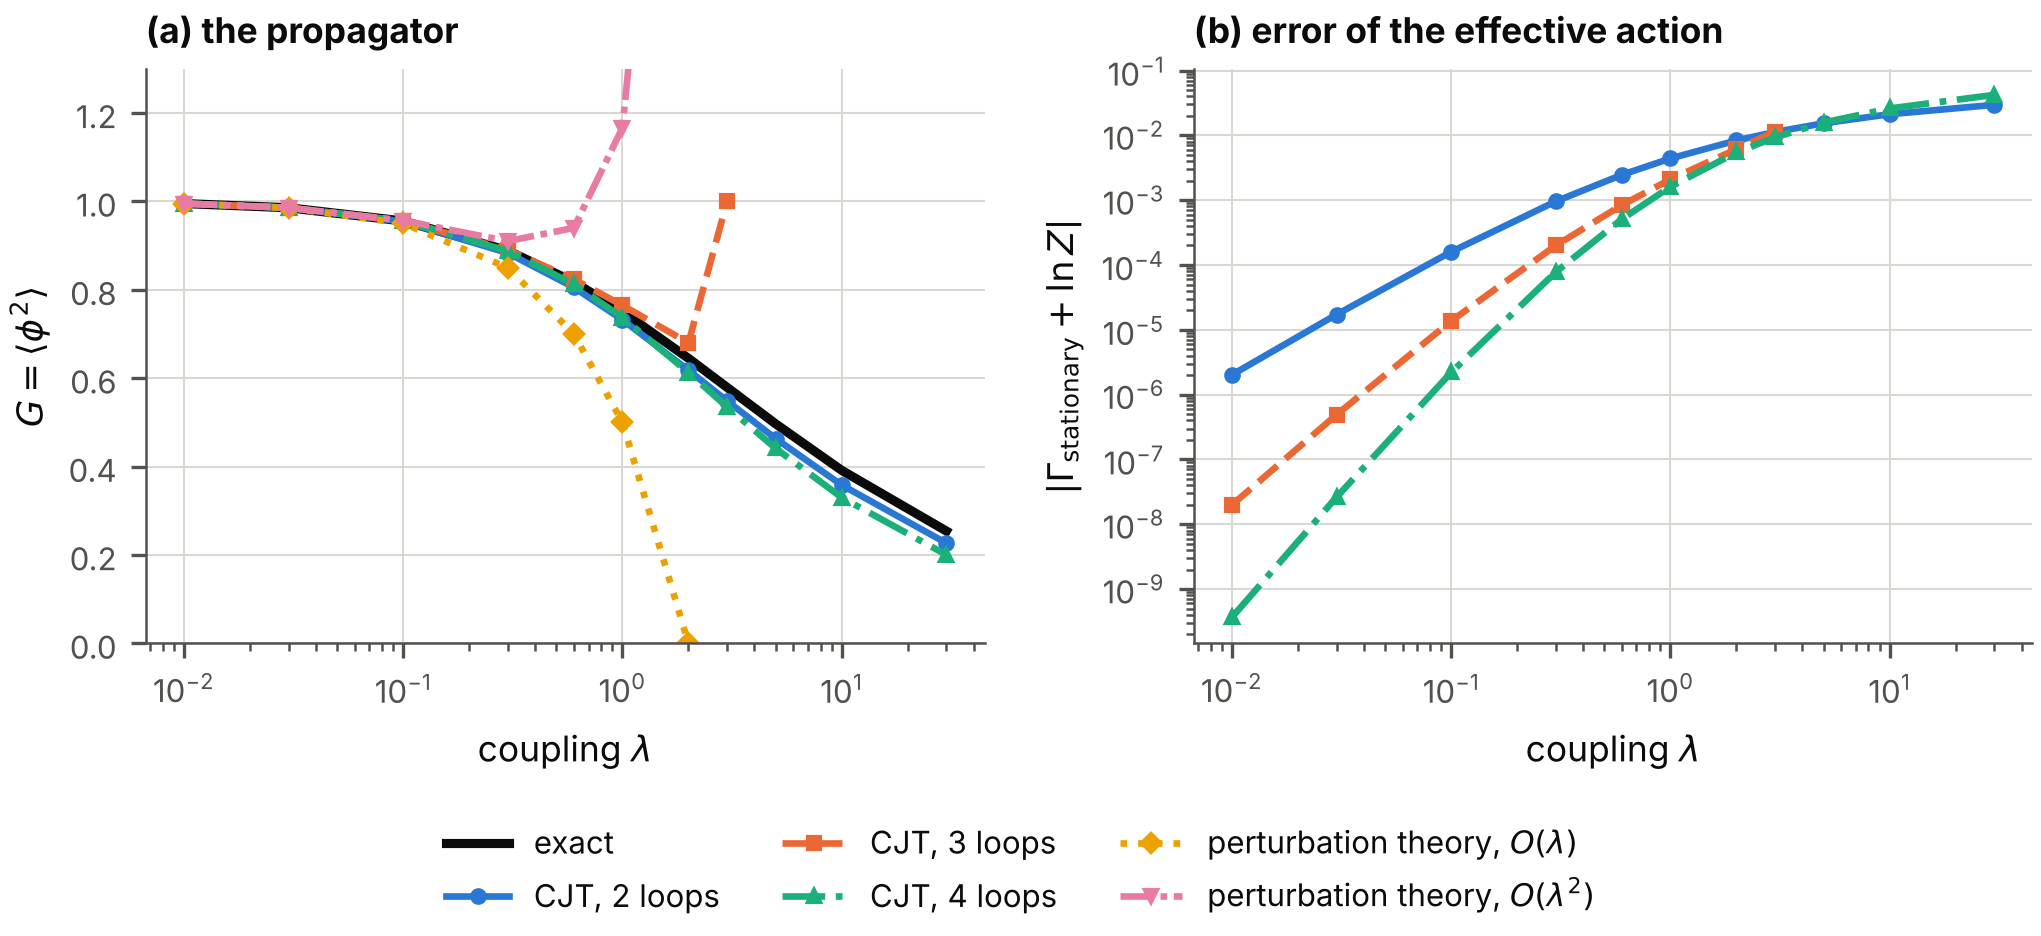
\includegraphics[width=1\textwidth,height=\textheight]{../figures/fig_cjt_toy.png}
\caption{The CJT method in zero dimensions. (a) The exact propagator,
the solutions of the gap equation with \(\Gamma_2\) truncated at two,
three and four loops, and ordinary perturbation theory. (b) Difference
between the effective action at the stationary point and the exact
\(-\ln Z\). Data: \texttt{data/cjt\_toy.csv}.}
\end{figure}

\begin{longtable}[]{@{}
  >{\raggedleft\arraybackslash}p{(\columnwidth - 16\tabcolsep) * \real{0.0820}}
  >{\raggedleft\arraybackslash}p{(\columnwidth - 16\tabcolsep) * \real{0.1148}}
  >{\raggedleft\arraybackslash}p{(\columnwidth - 16\tabcolsep) * \real{0.1148}}
  >{\raggedleft\arraybackslash}p{(\columnwidth - 16\tabcolsep) * \real{0.1148}}
  >{\raggedleft\arraybackslash}p{(\columnwidth - 16\tabcolsep) * \real{0.1148}}
  >{\raggedleft\arraybackslash}p{(\columnwidth - 16\tabcolsep) * \real{0.1148}}
  >{\raggedleft\arraybackslash}p{(\columnwidth - 16\tabcolsep) * \real{0.1148}}
  >{\raggedleft\arraybackslash}p{(\columnwidth - 16\tabcolsep) * \real{0.1148}}
  >{\raggedleft\arraybackslash}p{(\columnwidth - 16\tabcolsep) * \real{0.1148}}@{}}
\toprule\noalign{}
\begin{minipage}[b]{\linewidth}\raggedleft
\(\lambda\)
\end{minipage} & \begin{minipage}[b]{\linewidth}\raggedleft
exact
\end{minipage} & \begin{minipage}[b]{\linewidth}\raggedleft
2 loops
\end{minipage} & \begin{minipage}[b]{\linewidth}\raggedleft
3 loops
\end{minipage} & \begin{minipage}[b]{\linewidth}\raggedleft
4 loops
\end{minipage} & \begin{minipage}[b]{\linewidth}\raggedleft
5 loops
\end{minipage} & \begin{minipage}[b]{\linewidth}\raggedleft
pert. \(O(\lambda)\)
\end{minipage} & \begin{minipage}[b]{\linewidth}\raggedleft
\(O(\lambda^2)\)
\end{minipage} & \begin{minipage}[b]{\linewidth}\raggedleft
\(O(\lambda^3)\)
\end{minipage} \\
\midrule\noalign{}
\endhead
\bottomrule\noalign{}
\endlastfoot
0.1 & 0.9556 & 0.9545 & 0.9557 & 0.9555 & 0.9556 & 0.950 & 0.957 &
0.955 \\
0.3 & 0.8887 & 0.8830 & 0.8905 & 0.8878 & 0.8894 & 0.850 & 0.910 &
0.873 \\
0.6 & 0.8176 & 0.8054 & 0.8240 & 0.8125 & 0.8242 & 0.700 & 0.940 &
0.643 \\
1 & 0.7505 & 0.7321 & 0.7646 & 0.7373 & 0.9776 & 0.500 & 1.167 &
-0.208 \\
2 & 0.6449 & 0.6180 & 0.6801 & 0.6127 & --- & 0.000 & 2.667 & -8.333 \\
3 & 0.5792 & 0.5486 & 1.0000 & 0.5351 & --- & -0.500 & 5.500 &
-31.625 \\
5 & 0.4966 & 0.4633 & --- & 0.4411 & --- & -1.500 & 15.167 & -156.708 \\
10 & 0.3915 & 0.3583 & --- & 0.3300 & --- & -4.000 & 62.667 &
-1312.333 \\
\end{longtable}

Three lessons, which carry over to field theory:

\begin{enumerate}
\def\labelenumi{\arabic{enumi}.}
\tightlist
\item
  \textbf{The two-loop truncation is uniformly good.} It stays within 11
  per cent of the exact propagator for all couplings from 0.01 to 30,
  where the perturbation series is useless beyond \(\lambda\approx0.5\).
  (Its solution, \(G=(\sqrt{1+2\lambda}-1)/\lambda\), has the correct
  qualitative behaviour for \(\lambda\to\infty\).)
\item
  \textbf{More loops help only at weak coupling.} The series (1.11) is
  asymptotic, like the perturbation series. At \(\lambda=1\) the error
  of the effective action falls from \(4.4\times10^{-3}\) (two loops) to
  \(1.6\times10^{-3}\) (four loops). The truncations at three and at
  five loops, whose last term in \(\Sigma\) is negative, have no
  acceptable solution at all for \(\lambda\ge5\) and for \(\lambda\ge2\)
  respectively (dashes in the table; the entry 1.0000 at \(\lambda=3\)
  is a solution, but a poor one).
\item
  \textbf{The stationary value is more accurate than the propagator}, as
  stated in Sec. 1.6.
\end{enumerate}

The applications below use the two-loop truncation.

\begin{center}\rule{0.5\linewidth}{0.5pt}\end{center}

\hypertarget{the-cjt-action-of-the-two-models}{%
\section{2. The CJT action of the two
models}\label{the-cjt-action-of-the-two-models}}

\hypertarget{variables}{%
\subsection{2.1 Variables}\label{variables}}

The fields are the fermion field \(\psi\) and the complex Vorton-Scalar
\(\Phi_{VS}\) (S1, Eqs. (1.1) and (3.1)). The variables of the CJT
action are:

\begin{longtable}[]{@{}
  >{\raggedright\arraybackslash}p{(\columnwidth - 4\tabcolsep) * \real{0.1856}}
  >{\raggedright\arraybackslash}p{(\columnwidth - 4\tabcolsep) * \real{0.4227}}
  >{\raggedright\arraybackslash}p{(\columnwidth - 4\tabcolsep) * \real{0.3918}}@{}}
\toprule\noalign{}
\begin{minipage}[b]{\linewidth}\raggedright
Variable
\end{minipage} & \begin{minipage}[b]{\linewidth}\raggedright
Meaning
\end{minipage} & \begin{minipage}[b]{\linewidth}\raggedright
Its stationarity condition
\end{minipage} \\
\midrule\noalign{}
\endhead
\bottomrule\noalign{}
\endlastfoot
\(\phi\) & expectation value, \(\langle\Phi_{VS}\rangle=\phi/\sqrt2\)
(real by a choice of phase); the fermion mass is \(g_{VS}\phi\) & field
equation of the Vorton-Scalar in the state considered \\
\(D_s\), \(D_\vartheta\) & propagators of the radial and of the phase
mode & their gap equations (masses in a medium or at finite
temperature) \\
\(\mathcal S\) & propagator of the doubled fermion field: normal blocks
and pair blocks & normal blocks: mass and energy of the fermions; pair
blocks: the gap equation \\
\end{longtable}

The action is the sum of (1.5) for the two boson modes and (1.10) for
the fermions:
\[\begin{aligned}\Gamma[\phi,D_s,D_\vartheta,\mathcal S]={}&S_{\rm cl}[\phi]
+\frac12\sum_{i=s,\vartheta}\Big\{\mathrm{Tr}\ln D_i^{-1}+\mathrm{Tr}\big[D_{0i}^{-1}(\phi)D_i-1\big]\Big\}\\
&-\frac12\mathrm{Tr}\ln\mathcal S^{-1}-\frac12\mathrm{Tr}\big[\mathcal S_0^{-1}(\phi)\,\mathcal S-1\big]+\Gamma_2[\phi,D_s,D_\vartheta,\mathcal S].\end{aligned}\tag{2.1}\]

\hypertarget{the-two-loop-gamma_2}{%
\subsection{\texorpdfstring{2.2 The two-loop
\(\Gamma_2\)}{2.2 The two-loop \textbackslash Gamma\_2}}\label{the-two-loop-gamma_2}}

With the vertices of S1, Eq. (1.4), there are three kinds of 2PI diagram
with two loops:

\begin{itemize}
\tightlist
\item
  \textbf{(a) a closed fermion line with one boson line across it}, for
  each of the two modes. Its derivative with respect to the fermion
  propagator is the self-energy of a fermion that emits and reabsorbs a
  boson: the normal blocks give the exchange (Fock) energy of Sec. 5.4,
  the pair blocks give the pairing interaction of Secs. 3 and 4 and,
  without a medium, the ladder equation of Sec. 7. Its derivative with
  respect to a boson propagator is the fermion loop in the boson
  self-energy.
\item
  \textbf{(b) two boson loops touching at a four-boson vertex} (the
  ``double bubble''), from the quartic terms of the potential of the
  Vorton-Scalar. It gives the bosons masses that depend on the
  temperature (Sec. 6).
\item
  \textbf{(c) two three-boson vertices joined by three boson lines},
  proportional to \(\lambda_{VS}^2\phi^2\). It is omitted, as in the
  Hartree approximation.
\end{itemize}

No diagram is needed for the mean field of the Vorton-Scalar acting on
the fermions: that effect is contained in the dependence of
\(S_{\rm cl}\) and of \(\mathcal S_0^{-1}(\phi)\) on \(\phi\), and it
appears when \(\Gamma\) is varied with respect to \(\phi\) (Sec. 5).

\hypertarget{which-part-is-used-where}{%
\subsection{2.3 Which part is used
where}\label{which-part-is-used-where}}

\begin{longtable}[]{@{}
  >{\raggedright\arraybackslash}p{(\columnwidth - 6\tabcolsep) * \real{0.0543}}
  >{\raggedright\arraybackslash}p{(\columnwidth - 6\tabcolsep) * \real{0.2500}}
  >{\raggedright\arraybackslash}p{(\columnwidth - 6\tabcolsep) * \real{0.2826}}
  >{\raggedright\arraybackslash}p{(\columnwidth - 6\tabcolsep) * \real{0.4130}}@{}}
\toprule\noalign{}
\begin{minipage}[b]{\linewidth}\raggedright
Sec.
\end{minipage} & \begin{minipage}[b]{\linewidth}\raggedright
State
\end{minipage} & \begin{minipage}[b]{\linewidth}\raggedright
Variables kept
\end{minipage} & \begin{minipage}[b]{\linewidth}\raggedright
Further approximations
\end{minipage} \\
\midrule\noalign{}
\endhead
\bottomrule\noalign{}
\endlastfoot
3, 4 & paired state in a medium & pair blocks of \(\mathcal S\) & static
exchange; particles only; \(\phi\), \(D_i\) and the normal blocks at
their values without pairing \\
5 & unpaired state in a medium, \(T=0\) & \(\phi\); normal blocks of
\(\mathcal S\) & exchange energy to first order; bosons at tree level \\
6 & no medium, temperature \(T\) & \(\phi\), \(D_s\), \(D_\vartheta\) &
fermions at one loop; diagram (b) only \\
7 & vacuum & pair blocks of \(\mathcal S\), all four momentum components
& linearized; no change of the normal blocks \\
\end{longtable}

\hypertarget{the-symmetry-that-organizes-the-results}{%
\subsection{2.4 The symmetry that organizes the
results}\label{the-symmetry-that-organizes-the-results}}

In the sector used throughout (fields independent of the four extra
coordinates) the models have an internal symmetry that was computed for
this supplement from the matrices (S1, Sec. 2.1). The complete output of
the program:

\begin{longtable}[]{@{}
  >{\raggedright\arraybackslash}p{(\columnwidth - 4\tabcolsep) * \real{0.5443}}
  >{\raggedright\arraybackslash}p{(\columnwidth - 4\tabcolsep) * \real{0.2278}}
  >{\raggedright\arraybackslash}p{(\columnwidth - 4\tabcolsep) * \real{0.2278}}@{}}
\toprule\noalign{}
\begin{minipage}[b]{\linewidth}\raggedright
item (computed from the matrices)
\end{minipage} & \begin{minipage}[b]{\linewidth}\raggedright
7+1
\end{minipage} & \begin{minipage}[b]{\linewidth}\raggedright
4+4
\end{minipage} \\
\midrule\noalign{}
\endhead
\bottomrule\noalign{}
\endlastfoot
dimension of the commutant, momenta along x1 x2 x3 & 8 & 8 \\
dimension of the commutant, momenta along x0 x1 x2 x3 & 4 & 4 \\
dimension of the commutant, momenta along every space coordinate of the
model & 1 & 4 \\
dimension of the centre of the zero-mode commutant & 2 & 2 \\
\(\lVert P^2-1\rVert\) for the traceless central generator \(P\) & 0 &
0 \\
dimensions of the two ideals & {[}3, 3{]} & {[}3, 3{]} \\
structure constant \(\lvert f_{123}\rvert\) of each ideal (generators
with \(\mathrm{Tr}\,T_iT_j=2\delta_{ij}\)) & 1.000000000000
1.000000000000 & 1.000000000000 1.000000000000 \\
\(\lVert\sum_iT_i^2-\tfrac34\,(\text{projector})\rVert\) for each ideal
& 0 0 & \(2.2\times10^{-16}\) \(2.2\times10^{-16}\) \\
positive-energy states with P = +1 and P = -1 at a test momentum &
4.000000 4.000000 & 4.000000 4.000000 \\
the four vector pair operators \(C^-\gamma^a\), \(a\in\{0,5,6,7\}\),
transform among themselves: residual & 0 & \(3.1\times10^{-16}\) \\
\(\lvert\text{Casimir}-\tfrac34\rvert\) of each ideal on the four pair
operators & 0 0 & \(5.5\times10^{-17}\) \(5.5\times10^{-17}\) \\
fermion number of the pair operators & 2.000000 & 2.000000 \\
charge of the pair operators under the central generator P & 0 & 0 \\
number of invariant quadratic forms on the four pair operators & 1 &
1 \\
the invariant form (diagonal; axes 0 5 6 7; first entry 1) & +1.000000
+1.000000 +1.000000 +1.000000 & +1.000000 -1.000000 -1.000000
-1.000000 \\
largest off-diagonal entry of the invariant form & 0 &
\(2.2\times10^{-16}\) \\
complex dimension of the generators that mix particles with
antiparticles, \(\mu=0\) & 2 & 2 \\
the same with a chemical potential & 0 & 0 \\
\(\gamma^0\gamma^5\) & antihermitian; commutator with the dynamics 0 &
Hermitian; commutator with the dynamics 0 \\
\(\gamma^0\gamma^6\) & antihermitian; commutator with the dynamics 0 &
Hermitian; commutator with the dynamics 0 \\
\(\gamma^0\gamma^7\) & antihermitian; commutator with the dynamics 0 &
Hermitian; commutator with the dynamics 0 \\
\(\gamma^5\gamma^6\) & antihermitian; commutator with the dynamics 0 &
antihermitian; commutator with the dynamics 0 \\
\(\gamma^5\gamma^7\) & antihermitian; commutator with the dynamics 0 &
antihermitian; commutator with the dynamics 0 \\
\(\gamma^6\gamma^7\) & antihermitian; commutator with the dynamics 0 &
antihermitian; commutator with the dynamics 0 \\
\end{longtable}

All 24 items have the expected values
(\texttt{data/reduced\_symmetry.csv}, column \texttt{expected}; 24 of 24
flagged as correct by the program).

In words: the symmetry is
\(SU(2)_A\times SU(2)_B\times U(1)_F\times U(1)_E\) in both spacetimes;
the four vector pair operators form a 4-vector of
\(SO(4)=[SU(2)_A\times SU(2)_B]/Z_2\) with fermion number 2; and when
the chemical potential vanishes there are four more real generators,
which mix particles with antiparticles (the two lines before the last
six; Sec. 7.1). In 7+1 the \(SO(4)\) consists of rotations of the extra
space axes; in 4+4 half of its generators, the Hermitian matrices
\(\gamma^0\gamma^t\), have no geometric meaning.

\begin{center}\rule{0.5\linewidth}{0.5pt}\end{center}

\hypertarget{the-paired-state-checks-of-the-results-of-s1}{%
\section{3. The paired state: checks of the results of
S1}\label{the-paired-state-checks-of-the-results-of-s1}}

\hypertarget{the-potential}{%
\subsection{3.1 The potential}\label{the-potential}}

Keep in (2.1) the pair blocks of the fermion propagator and diagram (a),
with the three approximations of S1, Sec. 5.1 (static exchange;
particles only; the normal state unchanged). A propagator with pair
blocks is then specified by a gap function \(\Delta(k)\): the
quasi-particles have the energies \(E_k=\sqrt{\xi_k^2+\Delta(k)^2}\),
\(\xi_k=\sqrt{m^2+k^2}-\mu\), and the pair correlation is
\[\kappa(k)=\langle b(-\vec k)\,b(\vec k)\rangle=\frac{\Delta(k)}{2E_k}\tanh\frac{E_k}{2T}.\tag{3.1}\]
The sums over the Matsubara frequencies in (2.1) can be done in closed
form. For a unitary state (all \(\nu=8\) internal states have the same
gap), and measured from the unpaired state at the same \(T\) and
\(\mu\), the result is
\[\boxed{\;\begin{aligned}V[\Delta]={}&\nu\!\int\!\!\frac{d^3k}{(2\pi)^3}\Big\{\frac{|\xi_k|-E_k}{2}-T\ln\frac{1+e^{-E_k/T}}{1+e^{-|\xi_k|/T}}+\Delta(k)\,\kappa(k)\Big\}\\
&-\frac\nu2\int\!\!\frac{d^3k}{(2\pi)^3}\!\int\!\!\frac{d^3k'}{(2\pi)^3}\;\kappa(k)\,W(k,k')\,\kappa(k')\end{aligned}\;}\tag{3.2}\]
with the kernel \(W\) of S1, Eq. (5.3). The first line comes from the
trace terms of (1.10): the energy and the entropy of the
quasi-particles, and the term \(\Delta\kappa\) that the trace of
\(\mathcal S_0^{-1}\mathcal S\) contributes. The second line is
\(\Gamma_2\): one boson exchanged between two pairs. Because
\(\partial/\partial\Delta\) of the first two terms in the braces is
\(-\kappa\),
\[\frac{\delta V}{\delta\Delta(k)}=\nu\,\frac{\partial\kappa}{\partial\Delta}\,\Big[\Delta(k)-\int\!\!\frac{d^3k'}{(2\pi)^3}W(k,k')\,\kappa(k')\Big],\tag{3.3}\]
and \(\partial\kappa/\partial\Delta>0\): \textbf{the potential is
stationary exactly where the gap equation (5.2) of S1 holds.} The unit
test
\texttt{cjt\_pairing::tests::gradient\_against\_finite\_differences}
checks (3.3) against numerical derivatives of (3.2).

\hypertarget{four-checks}{%
\subsection{3.2 Four checks}\label{four-checks}}

The program evaluates (3.2) on the momentum grid of the command
\texttt{gap}, for twelve of its parameter sets: eight in the vector
channel, two each in the two-form channel and with the radial mode
alone.

\textbf{Check 1: an independent solution.} The gap equation is solved by
Newton's method with the exact Jacobian, starting from a function of
different height and shape (\texttt{Potential::newton}); the command
\texttt{gap} used fixed-point iteration. The two gap functions agree at
every grid point within \(1.1\times10^{-11}\) of the gap, and the gaps
stored in \texttt{data/gap\_scan.csv} within \(7.9\times10^{-9}\).

\textbf{Check 2: the solution is a minimum of the potential.} Along the
family \(s\,\Delta(k)\) of rescaled gap functions the potential has its
minimum at \(s=1\) (within \(5.1\times10^{-7}\)). All second variations
are positive: the matrix of second derivatives is
\(D^{1/2}(1-\tilde K)D^{1/2}\) with a positive diagonal matrix \(D\) and
\(\tilde K_{ij}=\sqrt{\omega_i\kappa_i'}\,W_{ij}\sqrt{\omega_j\kappa_j'}\)
(\(\omega_i\) the integration weights), and the smallest eigenvalue of
\(1-\tilde K\) is positive (column ``smallest curvature''; Cholesky
factorization and inverse iteration).

\textbf{Check 3: the value at the minimum} is the condensation energy.
In weak coupling it must approach \(V_{\rm BCS}=-\nu N(0)\Delta_F^2/4\),
with \(N(0)=k_FE_F'/2\pi^2\) the density of states per internal state
and \(\Delta_F\) the gap at the Fermi momentum. The ratio lies between
0.987 and 1.000, closest to 1 for the smallest gaps.

\textbf{Check 4: the critical temperature.} Below \(T_c\) the unpaired
state \(\Delta=0\) is unstable: the second variation of \(V\) there has
a negative direction. \(T_c\) is the temperature at which its
determinant changes sign (Gaussian elimination, bisection); it agrees
with the \(T_c\) of the linearized gap equation (power iteration in
\texttt{gap.rs}) within \(2.6\times10^{-12}\), the resolution of the
bisection.

In the table \(m_s\) and \(k_F\) are in units of the fermion mass \(m\);
``pair'' names the pair operator (S1, Sec. 6); the three columns of
differences are relative.

\begin{longtable}[]{@{}
  >{\raggedleft\arraybackslash}p{(\columnwidth - 20\tabcolsep) * \real{0.0698}}
  >{\raggedleft\arraybackslash}p{(\columnwidth - 20\tabcolsep) * \real{0.0698}}
  >{\raggedleft\arraybackslash}p{(\columnwidth - 20\tabcolsep) * \real{0.0698}}
  >{\raggedright\arraybackslash}p{(\columnwidth - 20\tabcolsep) * \real{0.0814}}
  >{\raggedleft\arraybackslash}p{(\columnwidth - 20\tabcolsep) * \real{0.1047}}
  >{\raggedleft\arraybackslash}p{(\columnwidth - 20\tabcolsep) * \real{0.1047}}
  >{\raggedleft\arraybackslash}p{(\columnwidth - 20\tabcolsep) * \real{0.1047}}
  >{\raggedleft\arraybackslash}p{(\columnwidth - 20\tabcolsep) * \real{0.1163}}
  >{\raggedleft\arraybackslash}p{(\columnwidth - 20\tabcolsep) * \real{0.0930}}
  >{\raggedleft\arraybackslash}p{(\columnwidth - 20\tabcolsep) * \real{0.0814}}
  >{\raggedleft\arraybackslash}p{(\columnwidth - 20\tabcolsep) * \real{0.1047}}@{}}
\toprule\noalign{}
\begin{minipage}[b]{\linewidth}\raggedleft
\(g_{VS}\)
\end{minipage} & \begin{minipage}[b]{\linewidth}\raggedleft
\(m_s\)
\end{minipage} & \begin{minipage}[b]{\linewidth}\raggedleft
\(k_F\)
\end{minipage} & \begin{minipage}[b]{\linewidth}\raggedright
pair
\end{minipage} & \begin{minipage}[b]{\linewidth}\raggedleft
gap\(/E_F\)
\end{minipage} & \begin{minipage}[b]{\linewidth}\raggedleft
Newton vs fixed point
\end{minipage} & \begin{minipage}[b]{\linewidth}\raggedleft
vs \texttt{gap\_scan.csv}
\end{minipage} & \begin{minipage}[b]{\linewidth}\raggedleft
\(V/V_{\rm BCS}\)
\end{minipage} & \begin{minipage}[b]{\linewidth}\raggedleft
smallest curvature
\end{minipage} & \begin{minipage}[b]{\linewidth}\raggedleft
\(T_c\)/gap
\end{minipage} & \begin{minipage}[b]{\linewidth}\raggedleft
\(T_c\): two methods
\end{minipage} \\
\midrule\noalign{}
\endhead
\bottomrule\noalign{}
\endlastfoot
2 & 0.3 & 0.5 & vector & \(5.84\times10^{-2}\) & \(3.3\times10^{-12}\) &
\(2.3\times10^{-9}\) & 0.9977 & 0.257 & 0.5660 &
\(2.6\times10^{-12}\) \\
2 & 0.3 & 1 & vector & \(1.38\times10^{-2}\) & \(4.8\times10^{-12}\) &
\(3.5\times10^{-9}\) & 0.9997 & 0.201 & 0.5668 &
\(2.6\times10^{-12}\) \\
2 & 1 & 1 & vector & \(5.03\times10^{-4}\) & \(1.1\times10^{-11}\) &
\(7.4\times10^{-9}\) & 1.0000 & 0.114 & 0.5669 &
\(2.6\times10^{-12}\) \\
2 & 0.1 & 1 & vector & \(3.42\times10^{-2}\) & \(2.8\times10^{-12}\) &
\(2.2\times10^{-9}\) & 0.9936 & 0.263 & 0.5641 &
\(2.6\times10^{-12}\) \\
3 & 1 & 0.35 & vector & \(3.68\times10^{-2}\) & \(5.7\times10^{-12}\) &
\(4.8\times10^{-9}\) & 0.9993 & 0.157 & 0.5666 &
\(2.6\times10^{-12}\) \\
3 & 1 & 0.5 & vector & \(5.84\times10^{-2}\) & \(4.7\times10^{-12}\) &
\(4.1\times10^{-9}\) & 0.9981 & 0.194 & 0.5660 &
\(2.6\times10^{-12}\) \\
3 & 1 & 1 & vector & \(6.86\times10^{-2}\) & \(4.1\times10^{-12}\) &
\(3.0\times10^{-9}\) & 0.9969 & 0.243 & 0.5655 &
\(2.6\times10^{-12}\) \\
3 & 0.3 & 1.5 & vector & \(1.28\times10^{-1}\) & \(3.2\times10^{-12}\) &
\(1.7\times10^{-9}\) & 0.9873 & 0.330 & 0.5634 &
\(2.6\times10^{-12}\) \\
2 & 0.3 & 0.5 & two-form & \(2.22\times10^{-2}\) & \(4.3\times10^{-12}\)
& \(3.1\times10^{-9}\) & 0.9997 & 0.219 & 0.5668 &
\(2.6\times10^{-12}\) \\
3 & 1 & 0.5 & two-form & \(3.20\times10^{-4}\) & \(1.0\times10^{-11}\) &
\(7.9\times10^{-9}\) & 1.0000 & 0.106 & 0.5669 &
\(2.6\times10^{-12}\) \\
2 & 0.3 & 0.5 & radial only & \(3.72\times10^{-2}\) &
\(3.7\times10^{-12}\) & \(2.5\times10^{-9}\) & 0.9991 & 0.239 & 0.5666 &
\(2.6\times10^{-12}\) \\
3 & 1 & 0.5 & radial only & \(9.38\times10^{-3}\) &
\(5.9\times10^{-12}\) & \(4.7\times10^{-9}\) & 0.9999 & 0.154 & 0.5669 &
\(2.6\times10^{-12}\) \\
\end{longtable}

\hypertarget{the-bound-pair-from-the-gap-equation}{%
\subsection{3.3 The bound pair, from the gap
equation}\label{the-bound-pair-from-the-gap-equation}}

Without a Fermi sea, at \(T=0\) and \(\mu<m\), the linearized gap
equation reads
\(\Delta(k)=\int\!\frac{d^3k'}{(2\pi)^3}W(k,k')\Delta(k')/[2(E_{k'}-\mu)]\).
With \(\psi=\Delta/[2(E-\mu)]\) and \(\mu=m-E_b/2\) it becomes, for
momenta small compared with \(m\),
\[\Big(\frac{k^2}{m}+E_b\Big)\psi(k)=\int\!\!\frac{d^3k'}{(2\pi)^3}\,W(k,k')\,\psi(k') :\]
the Schrödinger equation of the relative motion of two particles
(reduced mass \(m/2\)) with the potential \(-W\), which for the radial
mode is the Yukawa potential (4.6) of S1. \textbf{The instability of the
vacuum of pairs and the bound state of two particles are the same
thing}; this is how the paired state of overlapping pairs goes over into
a condensate of bound pairs (S1, Sec. 5.3). A bound state appears when
the largest eigenvalue of the kernel at \(\mu=m\) reaches 1. The program
finds the corresponding \(D_{VS}=\alpha_{VS}m/m_s\) with the
relativistic kernel:

\begin{longtable}[]{@{}
  >{\raggedleft\arraybackslash}p{(\columnwidth - 4\tabcolsep) * \real{0.2258}}
  >{\raggedleft\arraybackslash}p{(\columnwidth - 4\tabcolsep) * \real{0.3871}}
  >{\raggedleft\arraybackslash}p{(\columnwidth - 4\tabcolsep) * \real{0.3871}}@{}}
\toprule\noalign{}
\begin{minipage}[b]{\linewidth}\raggedleft
\(m_s/m\)
\end{minipage} & \begin{minipage}[b]{\linewidth}\raggedleft
\(D_c\) from the gap equation
\end{minipage} & \begin{minipage}[b]{\linewidth}\raggedleft
relative difference from \texttt{dimer.rs}
\end{minipage} \\
\midrule\noalign{}
\endhead
\bottomrule\noalign{}
\endlastfoot
0.3 & 1.73473 & +3.27e-02 \\
0.1 & 1.69016 & +6.16e-03 \\
0.03 & 1.68096 & +6.88e-04 \\
0.01 & 1.67994 & +8.13e-05 \\
0.003 & 1.67982 & +7.47e-06 \\
\end{longtable}

For a force of long range compared with the Compton wavelength of the
fermions the result is 1.67982; the program \texttt{dimer.rs}, which
integrates the radial Schrödinger equation in coordinate space, gave
1.67981. The two programs share no code. For \(m_s\) comparable to \(m\)
relativistic effects raise the threshold by a few per cent (first lines
of the table).

\hypertarget{the-ginzburglandau-coefficients}{%
\subsection{3.4 The Ginzburg--Landau
coefficients}\label{the-ginzburglandau-coefficients}}

Near \(T_c\) the potential can be expanded along a gap function of fixed
shape, \(\Delta(k)=s\,\varphi(k)\), where \(\varphi\) is the solution of
the linearized gap equation normalized to 1 at the Fermi momentum:
\(V=\alpha(T)\,s^2+\tfrac12\beta\,s^4+\dots\) For a unitary state
\(\mathrm{Tr}[\mathsf M\mathsf M^\dagger]=8s^2\), so that the
coefficients of S1, Sec. 6.2, are \(a=\alpha/8\) and \(b=\beta/8\).
Expanding (3.2) and using \(\int W\kappa'\varphi=\eta(T)\,\varphi\),
where \(\eta(T)\) is the largest eigenvalue of the linearized gap
equation (\(\eta(T_c)=1\)), one finds
\[\alpha(T)=\frac\nu2\big[1-\eta(T)\big]\!\int\!\!\frac{d^3k}{(2\pi)^3}\kappa'\varphi^2,\qquad
\frac\beta2=\nu\Big[\frac18-\frac{\eta(T)}{6}\Big]\!\int\!\!\frac{d^3k}{(2\pi)^3}\kappa'''\varphi^4,\tag{3.4}\]
with \(\kappa'\), \(\kappa'''\) the first and third derivatives of (3.1)
with respect to \(\Delta\) at \(\Delta=0\). At \(T_c\) the bracket of
\(\beta\) is \(-1/24\), and with a constant density of states (3.4)
gives the formulas of S1. Away from \(T_c\),
\(\eta(T)-1\approx-\lambda\ln(T/T_c)\) with \(\lambda=N(0)W\), so that
the coefficients of the potential along a fixed ray carry factors
\(1+O(\lambda\ln(T/T_c))\) --- for \(\beta\) the factor \(1+4(\eta-1)\).
The comparison is therefore made at \(T_c\) (the program fits \(V/s^2\)
at six small amplitudes for \(T/T_c=0.99\) and \(1.01\)). The gradient
coefficient \(K\) is obtained independently, from the dependence of the
pair susceptibility on the momentum of the pair
(\texttt{pair\_bubble\_curvature}).

\begin{longtable}[]{@{}
  >{\raggedleft\arraybackslash}p{(\columnwidth - 14\tabcolsep) * \real{0.0714}}
  >{\raggedleft\arraybackslash}p{(\columnwidth - 14\tabcolsep) * \real{0.0714}}
  >{\raggedleft\arraybackslash}p{(\columnwidth - 14\tabcolsep) * \real{0.0714}}
  >{\raggedleft\arraybackslash}p{(\columnwidth - 14\tabcolsep) * \real{0.1071}}
  >{\raggedleft\arraybackslash}p{(\columnwidth - 14\tabcolsep) * \real{0.1429}}
  >{\raggedleft\arraybackslash}p{(\columnwidth - 14\tabcolsep) * \real{0.1786}}
  >{\raggedleft\arraybackslash}p{(\columnwidth - 14\tabcolsep) * \real{0.1786}}
  >{\raggedleft\arraybackslash}p{(\columnwidth - 14\tabcolsep) * \real{0.1786}}@{}}
\toprule\noalign{}
\begin{minipage}[b]{\linewidth}\raggedleft
\(g_{VS}\)
\end{minipage} & \begin{minipage}[b]{\linewidth}\raggedleft
\(m_s/m\)
\end{minipage} & \begin{minipage}[b]{\linewidth}\raggedleft
\(k_F/m\)
\end{minipage} & \begin{minipage}[b]{\linewidth}\raggedleft
\(\lambda\)
\end{minipage} & \begin{minipage}[b]{\linewidth}\raggedleft
\(T_c/E_F\)
\end{minipage} & \begin{minipage}[b]{\linewidth}\raggedleft
\(a\): potential / formula
\end{minipage} & \begin{minipage}[b]{\linewidth}\raggedleft
\(b\): potential / formula
\end{minipage} & \begin{minipage}[b]{\linewidth}\raggedleft
\(K\): susceptibility / formula
\end{minipage} \\
\midrule\noalign{}
\endhead
\bottomrule\noalign{}
\endlastfoot
3 & 1 & 0.5 & 0.208 & \(3.3\times10^{-2}\) & 0.9993 & 0.9949 & 1.0101 \\
2 & 0.3 & 1 & 0.205 & \(7.8\times10^{-3}\) & 0.9998 & 0.9996 & 1.0007 \\
2 & 1 & 1 & 0.115 & \(2.9\times10^{-4}\) & 1.0000 & 1.0003 & 1.0000 \\
\end{longtable}

The three coefficients of S1 are confirmed within 1.0 per cent; the
deviations decrease with the coupling, as corrections of relative order
\(T_c/E_F\) and \(\lambda\) should. For the first parameter set the
temperature dependence is:

\begin{longtable}[]{@{}
  >{\raggedleft\arraybackslash}p{(\columnwidth - 4\tabcolsep) * \real{0.2000}}
  >{\raggedleft\arraybackslash}p{(\columnwidth - 4\tabcolsep) * \real{0.4000}}
  >{\raggedleft\arraybackslash}p{(\columnwidth - 4\tabcolsep) * \real{0.4000}}@{}}
\toprule\noalign{}
\begin{minipage}[b]{\linewidth}\raggedleft
\(T/T_c\)
\end{minipage} & \begin{minipage}[b]{\linewidth}\raggedleft
\(\alpha/[4N(0)\ln(T/T_c)]\)
\end{minipage} & \begin{minipage}[b]{\linewidth}\raggedleft
\(\beta/[7\zeta(3)N(0)/(2\pi^2T_c^2)]\)
\end{minipage} \\
\midrule\noalign{}
\endhead
\bottomrule\noalign{}
\endlastfoot
0.95 & 1.0099 & 1.1494 \\
0.98 & 1.0034 & 1.0530 \\
0.99 & 1.0013 & 1.0232 \\
1.01 & 0.9972 & 0.9667 \\
1.02 & 0.9951 & 0.9399 \\
1.05 & 0.9891 & 0.8650 \\
\end{longtable}

Both ratios pass through 1 at \(T_c\). The third column varies as
\((T_c/T)^2[1+4(\eta-1)]\), that is with the logarithmic slope
\(-(2+4\lambda)=\) -2.83 according to (3.4); the measured slope is
-2.84.

\begin{center}\rule{0.5\linewidth}{0.5pt}\end{center}

\hypertarget{the-paired-state-further-predictions}{%
\section{4. The paired state: further
predictions}\label{the-paired-state-further-predictions}}

\hypertarget{thermodynamics}{%
\subsection{4.1 Thermodynamics}\label{thermodynamics}}

At the solution of the gap equation, (3.2) is the difference of the
thermodynamic potentials of the paired and the unpaired state. Figure 2
and the table show it, together with the gap, the entropy \(S\) and the
heat capacity \(C=T\,dS/dT\), for \(g_{VS}=3\), \(m_s=m\),
\(k_F=0.5\,m\) in the vector channel (\(T_c/E_F=3.3\times10^{-2}\)).

\begin{figure}
\centering
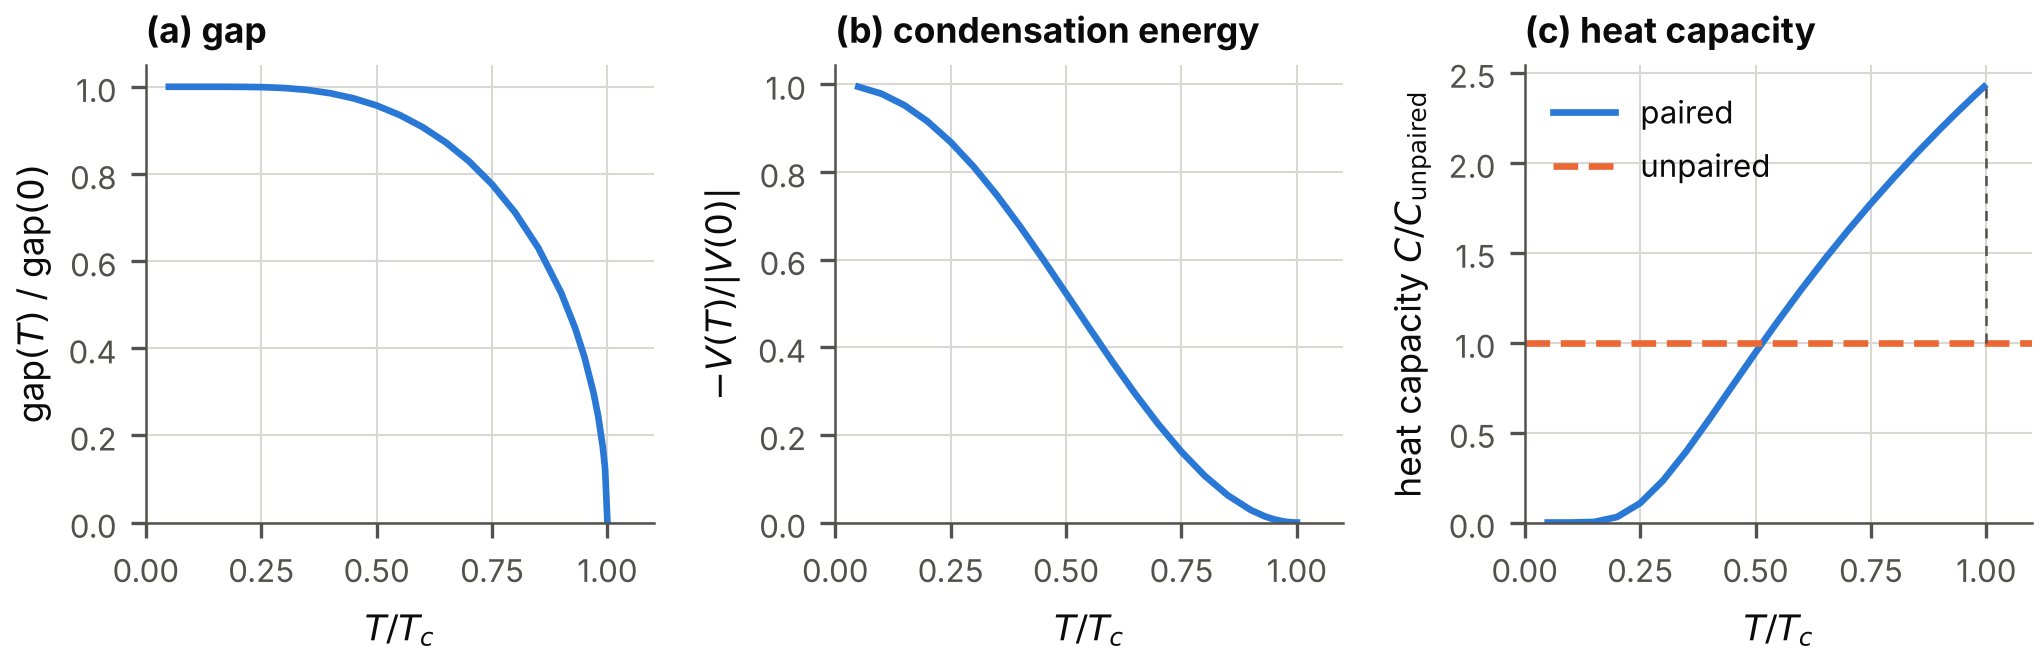
\includegraphics[width=1\textwidth,height=\textheight]{../figures/fig_cjt_thermo.png}
\caption{The paired state against temperature. (a) Gap at the Fermi
momentum. (b) Condensation energy (minus the CJT potential), in units of
its value at \(T=0\). (c) Heat capacity in units of that of the unpaired
state at the same temperature; it jumps at \(T_c\). Data:
\texttt{data/cjt\_thermo.csv}.}
\end{figure}

\begin{longtable}[]{@{}rrrrr@{}}
\toprule\noalign{}
\(T/T_c\) & gap\((T)\)/gap\((0)\) & \(-V(T)/|V(0)|\) & \(S_s/S_n\) &
\(C_s/C_n\) \\
\midrule\noalign{}
\endhead
\bottomrule\noalign{}
\endlastfoot
0.10 & 1.0000 & 0.9789 & 0.0000 & 0.0000 \\
0.20 & 0.9999 & 0.9156 & 0.0036 & 0.0304 \\
0.30 & 0.9971 & 0.8120 & 0.0409 & 0.2340 \\
0.40 & 0.9851 & 0.6766 & 0.1302 & 0.5743 \\
0.50 & 0.9570 & 0.5233 & 0.2561 & 0.9443 \\
0.60 & 0.9072 & 0.3675 & 0.4005 & 1.2973 \\
0.70 & 0.8291 & 0.2242 & 0.5521 & 1.6217 \\
0.80 & 0.7114 & 0.1071 & 0.7045 & 1.9170 \\
0.90 & 0.5266 & 0.0285 & 0.8544 & 2.1863 \\
0.95 & 0.3806 & 0.0073 & 0.9278 & 2.3123 \\
0.99 & 0.1731 & 0.0003 & 0.9857 & 2.4093 \\
\end{longtable}

The universal numbers of weak coupling are reproduced, with corrections
of the expected size for a gap of 6 per cent of the Fermi energy:
\[\begin{aligned}\frac{\Delta(0)}{T_c}&=1.7668\ (1.764),\qquad
\frac{C_s-C_n}{C_n}\Big|_{T_c}=1.433\ (1.426),\\
\frac{\Delta(T)}{T_c\sqrt{1-T/T_c}}\Big|_{0.98T_c}&=3.045\ (3.06\ \text{at}\ T_c).\end{aligned}\]
These hold for both spacetimes and for any unitary state. Two
consequences are used elsewhere: the entropy of the paired state is
exponentially small below about \(T_c/4\) (the paired fluid of
Supplement S3 is cold in the strict sense), and the condensation energy
per fermion, \(\tfrac38\Delta^2/E_F\) in the non-relativistic limit, is
a small fraction of the Fermi energy, so that pairing changes the
pressure by terms of relative order \((\Delta/E_F)^2\), as assumed in
S3, Sec. 4.1.

\hypertarget{the-space-of-the-order-parameter}{%
\subsection{4.2 The space of the order
parameter}\label{the-space-of-the-order-parameter}}

The order parameter has four complex components \(\Delta^a\) along the
extra axes \(a\in\{0,5,6,7\}\). The program builds the gap matrix
\(\mathsf M\) of S1, Eq. (6.1), from the Dirac matrices of each
spacetime and evaluates the CJT potential at \(T=0\) for a constant
attraction in each of the four channels (weak coupling;
\texttt{ShellModel}), in units in which the gap of the unitary state is
1 and \(N(0)=1\).

\textbf{The gaps of a general state.} In both spacetimes the eight
eigenvalues of \(\mathsf M\mathsf M^\dagger\) form two fourfold sets,
\[\boxed{\;d_\pm^2=\mathcal S\pm\sqrt{\mathcal S^2-\big|\eta_{ab}\Delta^a\Delta^b\big|^2},\qquad\mathcal S=\sum_a|\Delta^a|^2\;}\tag{4.1}\]
with the metric of the spacetime on the extra axes (unit test
\texttt{cjt\_pairing::tests::order\_parameter\_space}). The identity
(6.2) of S1 is the statement about \(d_+^4+d_-^4\) that follows from
(4.1); (4.1) is the complete statement. A state is unitary (\(d_+=d_-\))
when \(|\eta_{ab}\Delta^a\Delta^b|=\mathcal S\).

\begin{longtable}[]{@{}
  >{\raggedright\arraybackslash}p{(\columnwidth - 10\tabcolsep) * \real{0.0500}}
  >{\raggedright\arraybackslash}p{(\columnwidth - 10\tabcolsep) * \real{0.3250}}
  >{\raggedright\arraybackslash}p{(\columnwidth - 10\tabcolsep) * \real{0.1125}}
  >{\raggedleft\arraybackslash}p{(\columnwidth - 10\tabcolsep) * \real{0.0875}}
  >{\raggedright\arraybackslash}p{(\columnwidth - 10\tabcolsep) * \real{0.2125}}
  >{\raggedright\arraybackslash}p{(\columnwidth - 10\tabcolsep) * \real{0.2125}}@{}}
\toprule\noalign{}
\begin{minipage}[b]{\linewidth}\raggedright
\end{minipage} & \begin{minipage}[b]{\linewidth}\raggedright
state
\end{minipage} & \begin{minipage}[b]{\linewidth}\raggedright
the two gaps\(^2\)
\end{minipage} & \begin{minipage}[b]{\linewidth}\raggedleft
\(V\)
\end{minipage} & \begin{minipage}[b]{\linewidth}\raggedright
second derivatives
\end{minipage} & \begin{minipage}[b]{\linewidth}\raggedright
flat directions
\end{minipage} \\
\midrule\noalign{}
\endhead
\bottomrule\noalign{}
\endlastfoot
7+1 & hidden-axis singlet & 1.000, 1.000 & -2.0000 & 4 flat, 4 positive
(6.6647) & Im \(\Delta^0\) Re \(\Delta^5\) Re \(\Delta^6\) Re
\(\Delta^7\) \\
7+1 & along x5 & 1.000, 1.000 & -2.0000 & 4 flat, 4 positive (6.6647) &
Re \(\Delta^0\) Im \(\Delta^5\) Re \(\Delta^6\) Re \(\Delta^7\) \\
7+1 & unitary, rotated between x0 and x5 & 1.000, 1.000 & -2.0000 & 4
flat, 4 positive (6.6648) & (combinations) \\
7+1 & unitary, general direction and phase & 1.000, 1.000 & -2.0000 & 4
flat, 4 positive (6.6648) & (combinations) \\
7+1 & half-paired: \(\eta_{ab}\Delta^a\Delta^b\) = 0; larger gap 1 &
0.000, 1.000 & -1.0000 & stationary; unstable & --- \\
7+1 & the phases of the other signature's unitary state & 0.040, 1.960 &
-0.9184 & not stationary & --- \\
4+4 & hidden-axis singlet & 1.000, 1.000 & -2.0000 & 4 flat, 4 positive
(6.6647) & Im \(\Delta^0\) Im \(\Delta^5\) Im \(\Delta^6\) Im
\(\Delta^7\) \\
4+4 & along x5 & 1.000, 1.000 & -2.0000 & 4 flat, 4 positive (6.6647) &
Im \(\Delta^0\) Im \(\Delta^5\) Re \(\Delta^6\) Re \(\Delta^7\) \\
4+4 & unitary, rotated between x0 and x5 & 1.000, 1.000 & -2.0000 & 4
flat, 4 positive (6.6648) & (combinations) \\
4+4 & unitary, general direction and phase & 1.000, 1.000 & -2.0000 & 4
flat, 4 positive (6.6648) & (combinations) \\
4+4 & half-paired: \(\eta_{ab}\Delta^a\Delta^b\) = 0; larger gap 1 &
0.000, 1.000 & -1.0000 & stationary; unstable & --- \\
4+4 & the phases of the other signature's unitary state & 0.040, 1.960 &
-0.9184 & not stationary & --- \\
\end{longtable}

Reading the table:

\begin{enumerate}
\def\labelenumi{\arabic{enumi}.}
\tightlist
\item
  \textbf{The unitary states are the minima}, with \(V=-2\), that is
  \(-\nu N(0)\Delta^2/4\), whatever their direction: the hidden-axis
  singlet, a state along \(x5\), and rotated states have the same energy
  to the accuracy of the calculation, in both spacetimes.
\item
  \textbf{Four flat directions, four massive ones.} Around every unitary
  state four of the eight real directions cost no energy: the phase
  (fermion number) and three rotations of the direction (the breaking
  \(SO(4)\to SO(3)\)). They are the directions of the four gapless
  collective modes. The table shows which they are at the hidden-axis
  singlet: in 7+1 the imaginary part of \(\Delta^0\) and the \emph{real}
  parts of \(\Delta^5,\Delta^6,\Delta^7\); in 4+4 the imaginary part of
  \(\Delta^0\) and the \emph{imaginary} parts of the other three --- the
  hidden symmetry rotates \(\Delta^0\) into \(i\Delta^t\). The other
  four directions (the amplitude, and three that make the state
  non-unitary) have equal curvature, 6.6647 \(N(0)\).
\item
  \textbf{A half-paired stationary state.} If
  \(\eta_{ab}\Delta^a\Delta^b=0\), four of the eight internal states are
  paired with the full gap and four are not paired at all. The state is
  stationary and has half the condensation energy; it is unstable
  against opening the second gap (the potential rises by
  \(6.7\times10^{-4}\) when the order parameter is multiplied by 1.02 or
  by 0.98, and falls by \(2.1\times10^{-2}\) when 0.05 is added to
  \(\Delta^0\)). It is the analogue of the non-unitary phases of
  superfluid \(^3\)He, which are stabilized by a magnetic field; here
  the corresponding field would be a chemical potential for one of the
  generators of \(SO(4)\).
\item
  The configuration that is unitary in one spacetime is far from unitary
  in the other (last line of each block): the relative phase between
  \(\Delta^0\) and \(\Delta^5\) that minimizes the energy is 0 in 7+1
  and \(\pi/2\) in 4+4.
\end{enumerate}

The curvatures of the potential in the massive directions depend on how
propagators away from the stationary point are parametrized; they are
not frequencies of collective modes. The number of flat directions and
the energies of stationary states do not depend on that choice.

\textbf{Consequences.} Both models have, besides the sound mode, three
gapless modes in which the direction of the order parameter in the space
of the extra axes oscillates. In 7+1 they are exact Goldstone modes of
the model. In 4+4 they are protected by the hidden symmetry only; any
dependence of the fields on \(x0\) gives them a mass (S1, Sec. 6.3).

\begin{center}\rule{0.5\linewidth}{0.5pt}\end{center}

\hypertarget{the-unpaired-state-in-a-medium-what-the-vorton-scalar-does-to-the-fermion-mass}{%
\section{5. The unpaired state in a medium: what the Vorton-Scalar does
to the fermion
mass}\label{the-unpaired-state-in-a-medium-what-the-vorton-scalar-does-to-the-fermion-mass}}

\hypertarget{the-field-equation-in-matter}{%
\subsection{5.1 The field equation in
matter}\label{the-field-equation-in-matter}}

Vary (2.1) with respect to \(\phi\) for a Fermi sea without pairing at
\(T=0\). The fermion mass is \(m^*=g_{VS}\phi\); write \(x=m^*/m\). With
the tree-level potential of the Vorton-Scalar and the energy of fermions
of mass \(m^*\) filled up to the Fermi momentum \(k_F\) (density
\(n=\nu k_F^3/6\pi^2\)), the energy density in units of \(m^4\) is
\[\varepsilon(k_F,x)=\frac{(x^2-1)^2}{8C}+\nu\!\int_0^{k_F}\!\frac{k^2dk}{2\pi^2}\sqrt{k^2+x^2}\;\big[+V_{\rm sea}(x)\big],\quad
\boxed{C=\frac{g_{VS}^2m^2}{m_s^2}=\frac{g_{VS}^4}{2\lambda_{VS}}=4\pi D_{VS}\frac{m}{m_s}}\tag{5.1}\]
and stationarity in \(x\) is the field equation of the Vorton-Scalar
(S1, Eq. (1.8)) with the scalar density of the fermions as source:
\[x^2=1-2C\,\nu\!\int_0^{k_F}\!\frac{k^2dk}{2\pi^2}\frac{1}{\sqrt{k^2+x^2}}\quad\text{or}\quad x=0 .\tag{5.2}\]
\emph{Everything depends on the single number \(C\).} At low density
(5.2) gives \(m^*=m\,(1-C\,n/m^3)\): the mass falls linearly with the
density. The term in square brackets in (5.1) is the energy of the
filled negative-energy states, which changes when the mass changes. It
is divergent and must be renormalized; the symmetry \(U(1)_{VS}\) allows
two counterterms, which are fixed by requiring that the vacuum value and
the mass of the radial mode keep their tree-level values:
\[V_{\rm sea}(x)=-\frac{\nu}{32\pi^2}\Big[x^4\ln x^2-\frac32x^4+2x^2-\frac12\Big],\qquad V_{\rm sea}(1)=V_{\rm sea}'(1)=V_{\rm sea}''(1)=0.\tag{5.3}\]
Results are given without and with this term; the difference measures
how much depends on the quantum fluctuations of the fermions.

\hypertarget{results-the-abnormal-state-and-self-bound-matter}{%
\subsection{5.2 Results: the abnormal state, and self-bound
matter}\label{results-the-abnormal-state-and-self-bound-matter}}

\begin{figure}
\centering
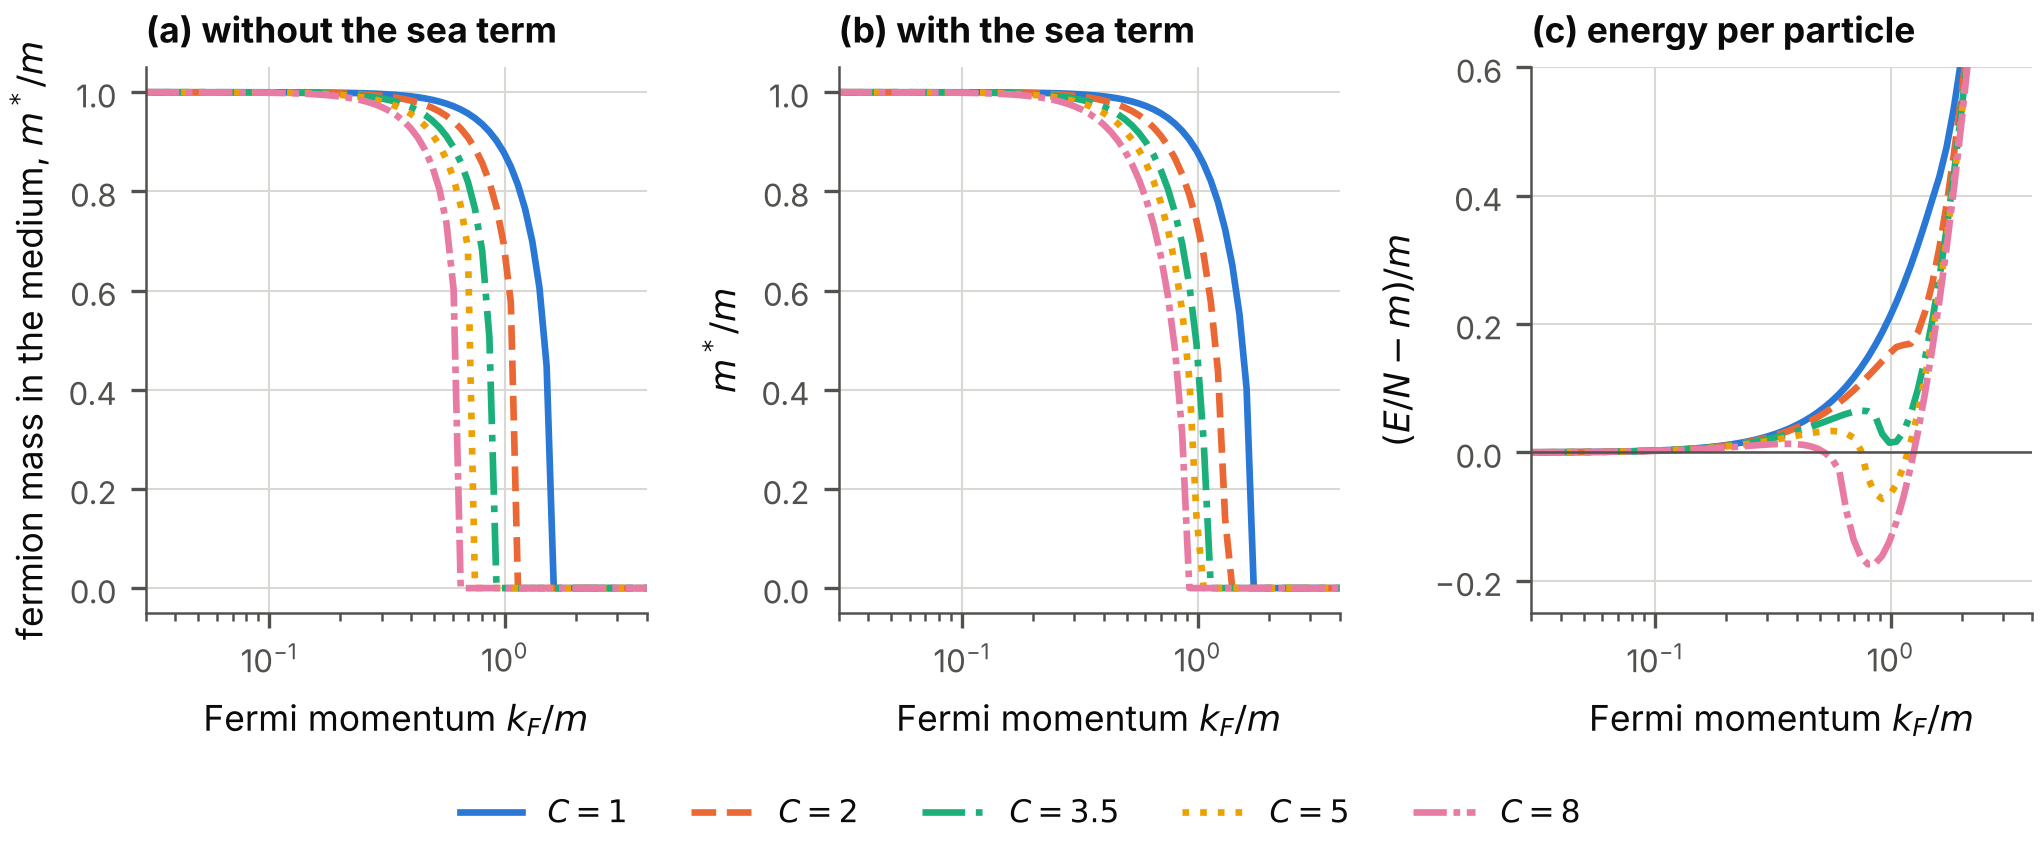
\includegraphics[width=1\textwidth,height=\textheight]{../figures/fig_cjt_normal.png}
\caption{The unpaired state at zero temperature. (a), (b) Fermion mass
in the medium against the Fermi momentum, without and with the energy of
the negative-energy states. (c) Energy per particle relative to the mass
of a free fermion; a minimum below zero means that matter is self-bound.
Data: \texttt{data/cjt\_normal.csv}.}
\end{figure}

\begin{longtable}[]{@{}
  >{\raggedleft\arraybackslash}p{(\columnwidth - 16\tabcolsep) * \real{0.0769}}
  >{\raggedleft\arraybackslash}p{(\columnwidth - 16\tabcolsep) * \real{0.1385}}
  >{\raggedleft\arraybackslash}p{(\columnwidth - 16\tabcolsep) * \real{0.1077}}
  >{\raggedleft\arraybackslash}p{(\columnwidth - 16\tabcolsep) * \real{0.1077}}
  >{\raggedleft\arraybackslash}p{(\columnwidth - 16\tabcolsep) * \real{0.1077}}
  >{\raggedleft\arraybackslash}p{(\columnwidth - 16\tabcolsep) * \real{0.1077}}
  >{\raggedleft\arraybackslash}p{(\columnwidth - 16\tabcolsep) * \real{0.1385}}
  >{\raggedleft\arraybackslash}p{(\columnwidth - 16\tabcolsep) * \real{0.1077}}
  >{\raggedleft\arraybackslash}p{(\columnwidth - 16\tabcolsep) * \real{0.1077}}@{}}
\toprule\noalign{}
\begin{minipage}[b]{\linewidth}\raggedleft
\(C\)
\end{minipage} & \begin{minipage}[b]{\linewidth}\raggedleft
\(E/N-m\)
\end{minipage} & \begin{minipage}[b]{\linewidth}\raggedleft
\(k_F^{\rm sat}\)
\end{minipage} & \begin{minipage}[b]{\linewidth}\raggedleft
\(k_F^{\rm abn}\)
\end{minipage} & \begin{minipage}[b]{\linewidth}\raggedleft
\(m^*/m\) before
\end{minipage} & \begin{minipage}[b]{\linewidth}\raggedleft
\(k_F^{\rm inst}\)
\end{minipage} & \begin{minipage}[b]{\linewidth}\raggedleft
with sea: \(E/N-m\)
\end{minipage} & \begin{minipage}[b]{\linewidth}\raggedleft
\(k_F^{\rm abn}\)
\end{minipage} & \begin{minipage}[b]{\linewidth}\raggedleft
\(k_F^{\rm inst}\)
\end{minipage} \\
\midrule\noalign{}
\endhead
\bottomrule\noalign{}
\endlastfoot
0.5 & not bound & --- & 2.226 & 0.10 & --- & not bound & 2.336 & --- \\
1 & not bound & --- & 1.576 & 0.17 & --- & not bound & 1.724 & --- \\
2 & not bound & --- & 1.123 & 0.35 & 1.023 & not bound & 1.317 & --- \\
3 & not bound & --- & 0.932 & 0.43 & 0.750 & not bound & 1.151 &
1.135 \\
3.5 & not bound & --- & 0.867 & 0.48 & 0.676 & not bound & 1.100 &
0.923 \\
4 & -0.019 & 0.981 & 0.818 & 0.50 & 0.589 & not bound & 1.059 & 0.776 \\
5 & -0.072 & 0.928 & 0.742 & 0.53 & 0.479 & not bound & 0.999 & 0.610 \\
6 & -0.114 & 0.886 & 0.688 & 0.55 & 0.403 & -0.002 & 0.955 & 0.479 \\
8 & -0.175 & 0.825 & 0.610 & 0.59 & 0.305 & -0.043 & 0.901 & 0.351 \\
12 & -0.255 & 0.745 & 0.516 & 0.64 & 0.209 & -0.091 & 0.840 & 0.224 \\
20 & -0.344 & 0.656 & 0.423 & 0.68 & 0.124 & -0.135 & 0.790 & 0.129 \\
35.5 & -0.432 & 0.568 & 0.340 & 0.71 & 0.072 & -0.168 & 0.755 & 0.072 \\
\end{longtable}

Columns: \(E/N-m\) lowest energy per particle of matter at any density
(in units of \(m\); ``not bound'' if it is not below zero);
\(k_F^{\rm sat}\) Fermi momentum of that state; \(k_F^{\rm abn}\) Fermi
momentum above which the stable state has \(m^*=0\), and \(m^*/m\) just
below it; \(k_F^{\rm inst}\) Fermi momentum above which the pressure
falls with increasing density. Momenta in units of \(m\).

\begin{enumerate}
\def\labelenumi{\arabic{enumi}.}
\tightlist
\item
  \textbf{Above a critical density the Vorton-Scalar has no expectation
  value and the fermions are massless.} This is the ``abnormal state''
  of matter that Lee and Wick predicted for any theory in which fermions
  obtain their mass from a scalar field. Without the sea term the mass
  jumps to zero (the jump is small for small \(C\)); with it the mass
  falls continuously, to the resolution of the scan. For weak coupling
  the transition is at \(k_F=\pi m/(2\sqrt C)\).
\item
  \textbf{Matter is self-bound if \(C\) exceeds a critical value}:
  \[C>\frac{3\pi^2}{8}=3.70\quad\text{(without sea term)},\qquad C>\frac{3\pi^2}{5}=5.92\quad\text{(with it)}.\]
  The program finds 3.7011 and 5.9218. The closed values follow from the
  energy of the abnormal state: massless fermions with pressure equal to
  the energy density \(B\) of the state without expectation value, as in
  the bag model of hadrons, have the energy per particle
  \((24\pi^2B/\nu)^{1/4}\), and \(B=m^4/8C\) at tree level,
  \(B=m^4/8C+\nu m^4/64\pi^2\) with (5.3). The bound state is always the
  abnormal one. For large \(C\) a fermion in matter weighs much less
  than a free one: 43 per cent less for \(C=35.5\) without the sea term,
  17 per cent with it.
\item
  \textbf{The dilute gas is mechanically unstable above a low density}
  (\(k_F^{\rm inst}\)). At low density the criterion is
  \(k_F>\pi^2m/4C\), or, in terms of the scattering length
  \(a=-g_{VS}^2m/4\pi m_s^2\) of the mean-field interaction,
  \(k_F|a|>\pi/16\).
\end{enumerate}

\hypertarget{a-warning-about-strong-coupling}{%
\subsection{5.3 A warning about strong
coupling}\label{a-warning-about-strong-coupling}}

The same function (5.3) shows that for field values \emph{larger} than
the vacuum value the one-loop potential of the Vorton-Scalar,
\((x^2-1)^2/8C+V_{\rm sea}(x)\), eventually decreases without bound: the
negative term \(x^4\ln x^2\) wins (for weak coupling when
\(\ln x^2>\tfrac32+4\pi^2/\nu C\)). The program locates the turning
points (\texttt{vacuum\_instability};
\texttt{data/cjt\_vacuum\_stability.csv}):

\begin{longtable}[]{@{}
  >{\raggedleft\arraybackslash}p{(\columnwidth - 4\tabcolsep) * \real{0.1795}}
  >{\raggedleft\arraybackslash}p{(\columnwidth - 4\tabcolsep) * \real{0.4103}}
  >{\raggedleft\arraybackslash}p{(\columnwidth - 4\tabcolsep) * \real{0.4103}}@{}}
\toprule\noalign{}
\begin{minipage}[b]{\linewidth}\raggedleft
\(C\)
\end{minipage} & \begin{minipage}[b]{\linewidth}\raggedleft
maximum of the potential at \(\phi/v_{VS}=\)
\end{minipage} & \begin{minipage}[b]{\linewidth}\raggedleft
below the vacuum beyond \(\phi/v_{VS}=\)
\end{minipage} \\
\midrule\noalign{}
\endhead
\bottomrule\noalign{}
\endlastfoot
0.1 & \(8.6\times10^{10}\) & \(1.1\times10^{11}\) \\
0.5 & 229 & 294 \\
1 & 19.3 & 24.7 \\
2 & 5.33 & 6.74 \\
3.7011 & 2.75 & 3.39 \\
5.9218 & 1.98 & 2.36 \\
10 & 1.54 & 1.77 \\
20 & 1.26 & 1.37 \\
35.5 & 1.14 & 1.21 \\
\end{longtable}

For \(C\ll1\), the regime of the weakly coupled superfluid, the
instability lies at exponentially large fields and is irrelevant. But
\textbf{the region of \(C\) in which matter is self-bound is a region in
which the model, taken at one loop, has no stable vacuum}: for
\(C\ge3.7\) the potential falls below its vacuum value at fields only
1.2 to 3.4 times the vacuum value (last column). There the model needs a
completion (a larger self-coupling, or new physics at that scale). This
is the analogue of the instability that a heavy fermion induces in the
potential of the Higgs field.

\hypertarget{the-exchange-energy}{%
\subsection{5.4 The exchange energy}\label{the-exchange-energy}}

The normal blocks of diagram (a) add the exchange (Fock) energy. To
first order (with the propagators of Sec. 5.1 and static exchange) it is
\[E_x=\frac{g_{VS}^2}{2}\,\frac\nu2\!\int\!\!\int_{k,k'<k_F}\!\frac{d^3k\,d^3k'}{(2\pi)^6}\;\frac{EE'\pm m^{*2}-\vec k\cdot\vec k'}{EE'}\;\frac{1}{|\vec k-\vec k'|^2+M^2},\]
upper sign and \(M=m_s\) for the radial mode, lower sign and \(M=0\) for
the phase mode (the factor in the middle is the trace of the two
vertices between the projectors on particle states). Both are positive.
In the limit of a heavy radial mode the first reduces to
\((g_{VS}^2/2m_s^2)(n^2+\rho_s^2)/2\nu\), the Fierz rearrangement of the
scalar interaction (unit test \texttt{fock\_energy\_contact\_limit}).

\begin{longtable}[]{@{}
  >{\raggedleft\arraybackslash}p{(\columnwidth - 12\tabcolsep) * \real{0.0909}}
  >{\raggedleft\arraybackslash}p{(\columnwidth - 12\tabcolsep) * \real{0.1136}}
  >{\raggedleft\arraybackslash}p{(\columnwidth - 12\tabcolsep) * \real{0.1364}}
  >{\raggedleft\arraybackslash}p{(\columnwidth - 12\tabcolsep) * \real{0.1136}}
  >{\raggedleft\arraybackslash}p{(\columnwidth - 12\tabcolsep) * \real{0.1364}}
  >{\raggedleft\arraybackslash}p{(\columnwidth - 12\tabcolsep) * \real{0.2045}}
  >{\raggedleft\arraybackslash}p{(\columnwidth - 12\tabcolsep) * \real{0.2045}}@{}}
\toprule\noalign{}
\begin{minipage}[b]{\linewidth}\raggedleft
\(C\)
\end{minipage} & \begin{minipage}[b]{\linewidth}\raggedleft
\(m_s/m\)
\end{minipage} & \begin{minipage}[b]{\linewidth}\raggedleft
\(g_{VS}^2\)
\end{minipage} & \begin{minipage}[b]{\linewidth}\raggedleft
\(k_F/m\)
\end{minipage} & \begin{minipage}[b]{\linewidth}\raggedleft
\(m^*/m\)
\end{minipage} & \begin{minipage}[b]{\linewidth}\raggedleft
radial mode (\%)
\end{minipage} & \begin{minipage}[b]{\linewidth}\raggedleft
phase mode (\%)
\end{minipage} \\
\midrule\noalign{}
\endhead
\bottomrule\noalign{}
\endlastfoot
2 & 0.3 & 0.18 & 0.1 & 1.000 & +11.1 & +0.3 \\
2 & 0.3 & 0.18 & 0.3 & 0.993 & +6.5 & +0.3 \\
2 & 0.3 & 0.18 & 0.6 & 0.943 & +3.1 & +0.3 \\
2 & 0.3 & 0.18 & 1 & 0.679 & +1.2 & +0.3 \\
2 & 1 & 2.00 & 0.1 & 1.000 & +12.4 & +3.1 \\
2 & 1 & 2.00 & 0.3 & 0.993 & +11.5 & +3.1 \\
2 & 1 & 2.00 & 0.6 & 0.943 & +9.4 & +3.2 \\
2 & 1 & 2.00 & 1 & 0.679 & +5.7 & +3.8 \\
2 & 3 & 18.00 & 0.1 & 1.000 & +12.5 & +28.1 \\
2 & 3 & 18.00 & 0.3 & 0.993 & +12.6 & +28.2 \\
2 & 3 & 18.00 & 0.6 & 0.943 & +12.5 & +29.1 \\
2 & 3 & 18.00 & 1 & 0.679 & +10.3 & +34.1 \\
5 & 1 & 5.00 & 0.1 & 0.999 & +12.4 & +3.1 \\
5 & 1 & 5.00 & 0.3 & 0.982 & +11.4 & +3.2 \\
5 & 1 & 5.00 & 0.6 & 0.832 & +8.4 & +3.6 \\
5 & 1 & 5.00 & 1 & 0.000 & +2.8 & +6.0 \\
\end{longtable}

The last two columns give the exchange energies in per cent of the
mean-field energy shift. The exchange of the radial mode reduces the
attraction by at most 12.6 per cent --- the factor \(1/\nu\) expected
for \(\nu=8\) internal states --- and less when the range of the force
exceeds the distance between the particles. The exchange of the phase
mode is of relative size \(2m_s^2/\nu^2m^2\) at low density: negligible
for a light radial mode, but larger than the radial term for \(m_s=3m\).
The thresholds of Sec. 5.2 are therefore accurate to about ten per cent
for \(m_s\lesssim m\), and the mean-field criterion for the instability
becomes \(k_F|a|>\pi/14\) when exchange is included (factor
\(1-1/\nu\)).

\hypertarget{consequences-for-the-dark-matter-analysis-of-s3}{%
\subsection{5.5 Consequences for the dark-matter analysis of
S3}\label{consequences-for-the-dark-matter-analysis-of-s3}}

\emph{Sound speed of the degenerate gas.} S3 used the sound speed of
free fermions. The mean field changes it by a factor \(1-O(k_F|a|)\).
Collisions of clusters of galaxies limit the scattering cross section
per mass to about 1 cm\(^2\)/g; with \(\sigma=4\pi a^2\) this gives
\(k_F|a|<\) \(6.4\times10^{-13}\) for fermions of 1 keV in a dwarf
galaxy. The correction is negligible, and the gas is far from the
instability of Sec. 5.2.

\emph{Bound clusters.} For the heavy, strongly coupled particles that S3
found to be acceptable cold dark matter (\(\alpha_{VS}=1\),
\(m\approx200\) MeV, \(m_s\approx120\) MeV), \(C=35.5\): large clusters
are self-bound and in the abnormal state, with 43 per cent of the rest
mass of the fermions radiated away as binding energy (17 per cent with
the sea term). Whether they form is a question of the history of the
early universe that is not addressed here; the warning of Sec. 5.3
applies to this regime.

\begin{center}\rule{0.5\linewidth}{0.5pt}\end{center}

\hypertarget{finite-temperature-the-fermion-mass-melts}{%
\section{6. Finite temperature: the fermion mass
melts}\label{finite-temperature-the-fermion-mass-melts}}

Without a medium of fermions but at a temperature \(T\) of the dark
sector, vary (2.1) with respect to \(\phi\) and to the two boson
propagators, with diagram (b) and the fermions at one loop
(\texttt{cjt\_normal.rs}, \texttt{Thermal}). The potential is
\[V=U_{\rm eff}(\phi)+\sum_{i=s,\vartheta}\Big[Q(M_i)+\frac12\big(a_i(\phi)-M_i^2\big)P(M_i)\Big]+\frac{\lambda_{VS}}{4}\big[3P_s^2+3P_\vartheta^2+2P_sP_\vartheta\big],\]
where \(U_{\rm eff}\) is the tree-level potential plus the fermion loop
(its vacuum part (5.3) and its thermal part), \(a_s=U_{\rm eff}''\),
\(a_\vartheta=U_{\rm eff}'/\phi\), \(P(M)\) is the thermal part of the
boson loop and \(Q(M)\) the thermal part of \(\tfrac12\mathrm{Tr}\ln\).
The last term is diagram (b). Stationarity in the masses gives the gap
equations \(M_s^2=a_s+3\lambda_{VS}P_s+\lambda_{VS}P_\vartheta\) and
\(M_\vartheta^2=a_\vartheta+\lambda_{VS}P_s+3\lambda_{VS}P_\vartheta\).

Two closed estimates of the temperature at which the expectation value
vanishes follow from the curvature of the potential at \(\phi=0\):
\[T_{\rm high}^2=\frac{12\,[\lambda_{VS}v_{VS}^2+\nu g_{VS}^2m^2/8\pi^2]}{4\lambda_{VS}+\nu g_{VS}^2},\qquad
T_N^2=\frac{12\,[\lambda_{VS}v_{VS}^2+\nu g_{VS}^2m^2/8\pi^2]}{2\lambda_{VS}+\nu g_{VS}^2}.\tag{6.1}\]
The first is the one-loop result at high temperature; the second
replaces the boson loops by their form for a large number of components,
in which the phase mode stays massless. The program follows the state of
lowest potential and determines the temperature \(T_{1/2}\) at which the
expectation value has fallen to half its vacuum value.

\begin{figure}
\centering
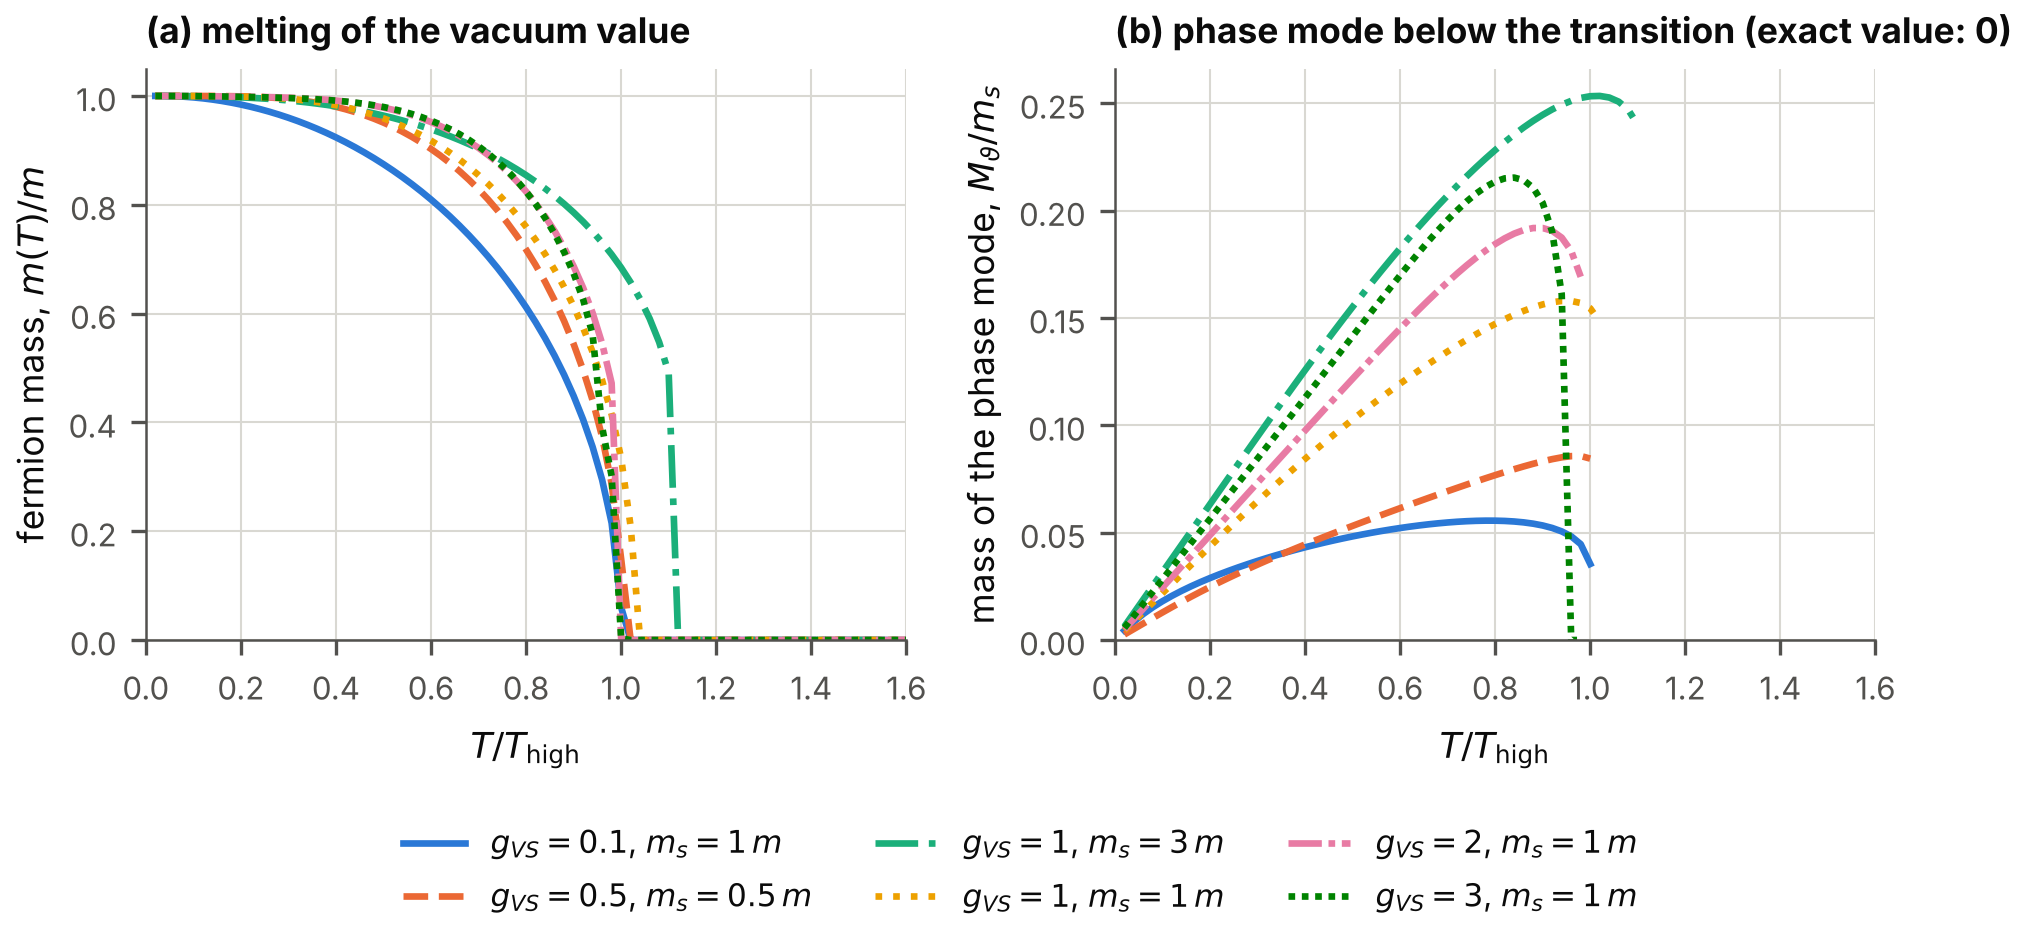
\includegraphics[width=1\textwidth,height=\textheight]{../figures/fig_cjt_thermal.png}
\caption{Finite temperature. (a) The expectation value of the
Vorton-Scalar, that is the fermion mass in units of its vacuum value, in
the state of lowest potential. (b) The mass that the Hartree
approximation gives to the phase mode below the transition; in the exact
theory it vanishes. Data: \texttt{data/cjt\_thermal\_profile.csv}.}
\end{figure}

\begin{longtable}[]{@{}
  >{\raggedleft\arraybackslash}p{(\columnwidth - 16\tabcolsep) * \real{0.0820}}
  >{\raggedleft\arraybackslash}p{(\columnwidth - 16\tabcolsep) * \real{0.0820}}
  >{\raggedleft\arraybackslash}p{(\columnwidth - 16\tabcolsep) * \real{0.0984}}
  >{\raggedleft\arraybackslash}p{(\columnwidth - 16\tabcolsep) * \real{0.1148}}
  >{\raggedleft\arraybackslash}p{(\columnwidth - 16\tabcolsep) * \real{0.1148}}
  >{\raggedleft\arraybackslash}p{(\columnwidth - 16\tabcolsep) * \real{0.1148}}
  >{\raggedleft\arraybackslash}p{(\columnwidth - 16\tabcolsep) * \real{0.1148}}
  >{\raggedleft\arraybackslash}p{(\columnwidth - 16\tabcolsep) * \real{0.1639}}
  >{\raggedleft\arraybackslash}p{(\columnwidth - 16\tabcolsep) * \real{0.1148}}@{}}
\toprule\noalign{}
\begin{minipage}[b]{\linewidth}\raggedleft
\(g_{VS}\)
\end{minipage} & \begin{minipage}[b]{\linewidth}\raggedleft
\(m_s/m\)
\end{minipage} & \begin{minipage}[b]{\linewidth}\raggedleft
\(C\)
\end{minipage} & \begin{minipage}[b]{\linewidth}\raggedleft
\(T_{\rm high}/v\)
\end{minipage} & \begin{minipage}[b]{\linewidth}\raggedleft
\(T_{N}/v\)
\end{minipage} & \begin{minipage}[b]{\linewidth}\raggedleft
\(T_{1/2}/v\)
\end{minipage} & \begin{minipage}[b]{\linewidth}\raggedleft
\(T_0/v\)
\end{minipage} & \begin{minipage}[b]{\linewidth}\raggedleft
\(\phi/v\) before \(T_0\)
\end{minipage} & \begin{minipage}[b]{\linewidth}\raggedleft
\(T_{1/2}/m\)
\end{minipage} \\
\midrule\noalign{}
\endhead
\bottomrule\noalign{}
\endlastfoot
0.1 & 1 & 0.01 & 0.775 & 0.817 & 0.677 & 0.776 & 0.07 & 6.77 \\
0.3 & 1 & 0.09 & 0.782 & 0.824 & 0.698 & 0.788 & 0.08 & 2.33 \\
0.5 & 0.5 & 1 & 0.461 & 0.468 & 0.423 & 0.464 & 0.08 & 0.85 \\
1 & 3 & 0.111 & 1.457 & 1.802 & 1.599 & 1.632 & 0.41 & 1.60 \\
1 & 1 & 1 & 0.849 & 0.895 & 0.808 & 0.875 & 0.10 & 0.81 \\
2 & 1 & 4 & 1.042 & 1.099 & 1.014 & 1.042 & 0.37 & 0.51 \\
3 & 1 & 9 & 1.302 & 1.372 & 1.238 & 1.302 & 0.14 & 0.41 \\
\end{longtable}

Columns: \(T_{1/2}\) temperature at which the expectation value has
fallen to half; \(T_0\) temperature at which it has fallen to zero
(below 2 per cent of \(v_{VS}\), the resolution of the scan); \(\phi/v\)
at \(0.998\,T_0\).

\begin{enumerate}
\def\labelenumi{\arabic{enumi}.}
\tightlist
\item
  \textbf{The fermion mass melts} at a temperature of order \(v_{VS}\):
  \(T_{1/2}\) agrees with the two estimates (6.1) within 17 per cent. In
  units of the fermion mass it ranges from 0.4 (strong Yukawa coupling)
  to 7 (weak).
\item
  \textbf{The order of the transition is not reliably predicted.} For
  the sets \((g_{VS},m_s/m)=\) (1, 3), (2, 1) the expectation value
  jumps to zero from about 0.4 \(v_{VS}\); for the others it falls
  steeply but, as far as the scan can tell, continuously (a square-root
  law, \(\phi/v_{VS}=\sqrt{1-T^2/T_0^2}\), gives 0.06 at \(0.998\,T_0\);
  the table has 0.07 to 0.14). The Hartree approximation is known to
  give a discontinuous transition for a pure scalar theory, where the
  true transition is continuous; a jump found here is therefore not
  evidence that the transition of the model is discontinuous. The table
  records what the truncated equations give.
\item
  \textbf{The defect of the approximation is visible} in panel (b):
  below the transition the phase mode has a mass of up to 0.25 \(m_s\)
  where Goldstone's theorem requires zero (Sec. 1.6).
\end{enumerate}

\emph{Consequence for the Hubble-tension analysis of S3.} There the
fermions annihilate when the temperature falls below about \(m/3\), at
constant mass. This is justified if the mass is already at its vacuum
value then, \(T_{1/2}\gg m/3\), which holds for \(g_{VS}\lesssim0.3\)
(first two lines of the table). For \(g_{VS}\gtrsim1\) the fermions
acquire their mass at a temperature below \(m\) and annihilate at once:
the step of the dark radiation would coincide with the transition. That
case was not simulated; since the simulated steps are already excluded,
it would not change the verdict unless the transition released the
entropy much earlier than the simulated range, in which case the
early-step family of S3 applies.

\begin{center}\rule{0.5\linewidth}{0.5pt}\end{center}

\hypertarget{the-vacuum-can-the-pair-condense-without-a-medium}{%
\section{7. The vacuum: can the pair condense without a
medium?}\label{the-vacuum-can-the-pair-condense-without-a-medium}}

\hypertarget{the-symmetry-without-a-chemical-potential}{%
\subsection{7.1 The symmetry without a chemical
potential}\label{the-symmetry-without-a-chemical-potential}}

When \(\mu=0\) the sector of fields independent of the extra coordinates
has more symmetry than in a medium: four further real generators exist,
which mix the field with its conjugate (computed in
\texttt{symmetry.rs}; Sec. 2.4). The reason is that the 16 components
are equivalent to four ordinary Dirac fields, or eight Majorana fields,
with equal masses; the radial mode couples to all eight alike, the phase
mode with opposite signs to the four with \(P=+1\) and the four with
\(P=-1\). The symmetry is \(O(4)\times O(4)\), of dimension 12. The pair
condensate of fermion number 2 is one orientation of a 16-component real
multiplet that also contains particle--antiparticle condensates; a
chemical potential reduces the symmetry to the \(U(2)\times U(2)\) of
Sec. 2.4 and singles out the pairs. Whatever its orientation, the
condensate does the same thing to the spectrum: it splits the masses of
two combinations of fields into \(m+\sigma\) and \(m-\sigma\).

\hypertarget{the-ladder-equation}{%
\subsection{7.2 The ladder equation}\label{the-ladder-equation}}

The stationarity condition of (2.1) for the fermion propagator with
diagram (a), in four-dimensional Euclidean momentum space, is
\[2\sigma(p)=g_{VS}^2\!\int\!\!\frac{d^4k}{(2\pi)^4}\big[f(m+\sigma)-f(m-\sigma)\big]\Big[\frac{1}{(p-k)^2+m_s^2}+\frac{1}{(p-k)^2}\Big],\qquad f(M)=\frac{M}{k^2+M^2}.\tag{7.1}\]
Both modes contribute with the same sign in this channel, as in the
medium. This is the ``ladder'' (or ``rainbow'') approximation that CJT
themselves used for dynamical symmetry breaking. Linearized in
\(\sigma\), after the angular integration, it is an eigenvalue problem
with the kernel
\(\frac{g_{VS}^2}{8\pi^2}\,k^3\frac{k^2-m^2}{(k^2+m^2)^2}\,[A(p,k;m_s)+A(p,k;0)]\),
\(A=2/[p^2+k^2+M^2+\sqrt{(p^2+k^2+M^2)^2-4p^2k^2}]\), and a cutoff
\(\Lambda\) where the four-dimensional description ends. A condensate
forms when the largest eigenvalue exceeds 1.

\emph{Test.} For massless fermions, one massless boson and momenta
between \(\mu\) and \(\Lambda\) the equation is solved by
\(\sigma\propto p^{-1}\cos(\rho\ln p^2+\delta)\), and the smallest
critical coupling is \(g^2/16\pi^2=\tfrac14+\rho^2\) with
\(\rho\ln(\Lambda/\mu)=\arctan(1/2\rho)\). The program reproduces this
within 0.2 per cent (unit test
\texttt{cjt\_vacuum::tests::scale\_invariant\_ladder\_equation}). With
two massless bosons and \(\Lambda\to\infty\) the critical coupling is
\(g^2/8\pi^2=\tfrac14\), that is \(\alpha_c=\pi/2\).

\begin{figure}
\centering
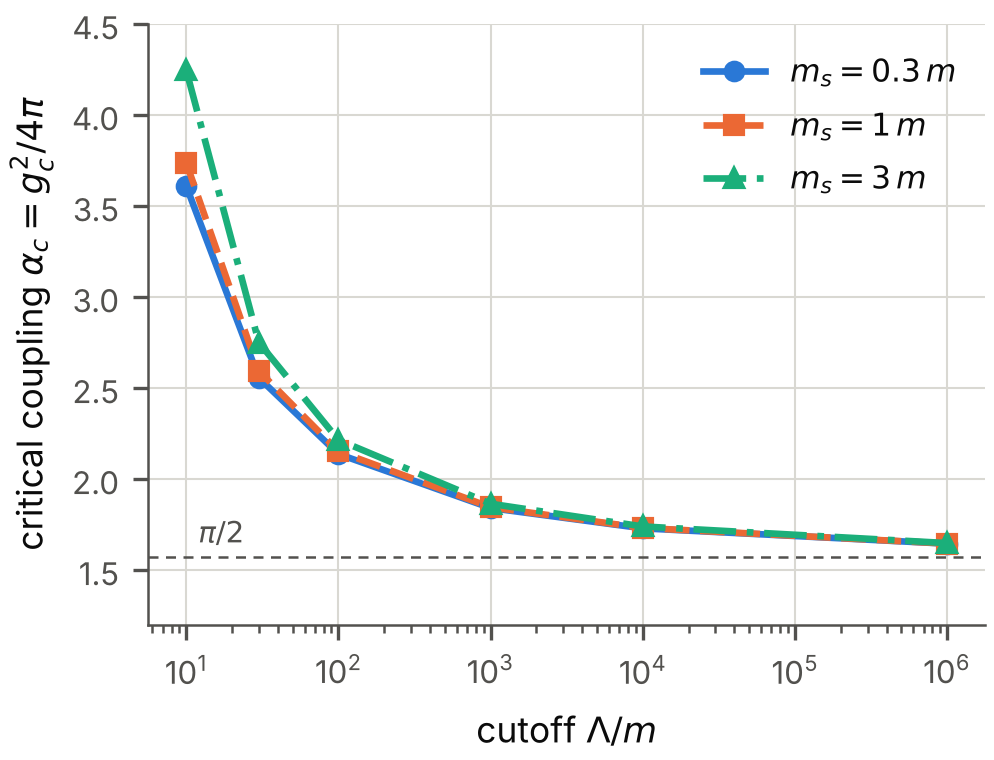
\includegraphics[width=0.55\textwidth,height=\textheight]{../figures/fig_cjt_vacuum.png}
\caption{Critical coupling for a pair condensate in the vacuum, against
the cutoff. Data: \texttt{data/cjt\_vacuum.csv}.}
\end{figure}

\begin{longtable}[]{@{}
  >{\raggedleft\arraybackslash}p{(\columnwidth - 12\tabcolsep) * \real{0.1250}}
  >{\raggedleft\arraybackslash}p{(\columnwidth - 12\tabcolsep) * \real{0.1458}}
  >{\raggedleft\arraybackslash}p{(\columnwidth - 12\tabcolsep) * \real{0.1458}}
  >{\raggedleft\arraybackslash}p{(\columnwidth - 12\tabcolsep) * \real{0.1458}}
  >{\raggedleft\arraybackslash}p{(\columnwidth - 12\tabcolsep) * \real{0.1458}}
  >{\raggedleft\arraybackslash}p{(\columnwidth - 12\tabcolsep) * \real{0.1458}}
  >{\raggedleft\arraybackslash}p{(\columnwidth - 12\tabcolsep) * \real{0.1458}}@{}}
\toprule\noalign{}
\begin{minipage}[b]{\linewidth}\raggedleft
\(m_s/m\)
\end{minipage} & \begin{minipage}[b]{\linewidth}\raggedleft
\(\Lambda/m=10^{1}\)
\end{minipage} & \begin{minipage}[b]{\linewidth}\raggedleft
\(\Lambda/m=30\)
\end{minipage} & \begin{minipage}[b]{\linewidth}\raggedleft
\(\Lambda/m=10^{2}\)
\end{minipage} & \begin{minipage}[b]{\linewidth}\raggedleft
\(\Lambda/m=10^{3}\)
\end{minipage} & \begin{minipage}[b]{\linewidth}\raggedleft
\(\Lambda/m=10^{4}\)
\end{minipage} & \begin{minipage}[b]{\linewidth}\raggedleft
\(\Lambda/m=10^{6}\)
\end{minipage} \\
\midrule\noalign{}
\endhead
\bottomrule\noalign{}
\endlastfoot
0.3 & 3.609 & 2.556 & 2.137 & 1.840 & 1.728 & 1.644 \\
1 & 3.737 & 2.593 & 2.152 & 1.844 & 1.730 & 1.645 \\
3 & 4.246 & 2.749 & 2.214 & 1.863 & 1.739 & 1.647 \\
\end{longtable}

\textbf{A pair condensate in the vacuum requires
\(\alpha_{VS}>\alpha_c\), between 1.64 and about 4 depending on the
cutoff.} For comparison: two fermions bind for
\(D_{VS}=\alpha_{VS}m/m_s>1.68\), so at such couplings bound pairs exist
unless \(m_s\gtrsim m\); and by Sec. 5.3 the one-loop potential of the
Vorton-Scalar is then unstable unless its self-coupling is equally
strong. The ladder approximation neglects the corrections to the
vertices and to the boson propagators, which are not small at these
couplings. The result is a statement about where to look, not a proof
that a condensate forms.

\emph{Consequence for the Higgs hypothesis (S2).} The condition ``the
condensate exists in empty space'' can be met only in a strongly coupled
Vorton-Scalar sector. This replaces a cruder estimate in an earlier
draft of S2 (error log E28).

\begin{center}\rule{0.5\linewidth}{0.5pt}\end{center}

\hypertarget{what-has-been-established-and-what-has-not}{%
\section{8. What has been established, and what has
not}\label{what-has-been-established-and-what-has-not}}

\textbf{Established:}

\begin{enumerate}
\def\labelenumi{\arabic{enumi}.}
\tightlist
\item
  The numerical results of S1 for the paired state --- gap functions,
  critical temperatures, condensation energy, the critical coupling of
  the bound pair, and the three Ginzburg--Landau coefficients --- are
  reproduced by a different formulation (the CJT potential) and
  different algorithms, to the accuracies of the table in Sec. 0.
\item
  The paired solution is a minimum of the potential; the unpaired state
  is unstable below \(T_c\).
\item
  The spectrum of gaps of a general state, Eq. (4.1); the manifold of
  ground states; four flat directions; the half-paired stationary state
  --- for both spacetimes, from their matrices.
\item
  Within the mean-field treatment: the fermion mass in matter, the
  abnormal state, the thresholds \(3\pi^2/8\) and \(3\pi^2/5\) for
  self-bound matter, and the size of the exchange corrections.
\item
  Within the Hartree approximation: the melting temperature of the
  fermion mass, to about 20 per cent.
\item
  Within the ladder approximation: the critical coupling for a vacuum
  condensate.
\end{enumerate}

\textbf{Not established:}

\begin{enumerate}
\def\labelenumi{\arabic{enumi}.}
\tightlist
\item
  Everything beyond the two-loop truncation of \(\Gamma_2\), and beyond
  the further approximations listed in Sec. 2.3. In particular the
  frequency dependence of the pairing interaction (the phase mode is
  massless, and its exchange is not instantaneous), which is known to
  change the prefactor of the gap in comparable systems.
\item
  The order of the thermal transition (Sec. 6), and all properties of
  the strong-coupling regime (Secs. 5.3 and 7).
\item
  The frequencies and dampings of the collective modes; only their
  number and the static energies were determined.
\item
  The masses that the three additional gapless modes of 4+4 acquire when
  the fields depend on \(x0\).
\item
  Paired states in the abnormal phase, and the pairing of massless
  fermions.
\end{enumerate}

\begin{center}\rule{0.5\linewidth}{0.5pt}\end{center}

\hypertarget{provenance-of-the-numbers-and-figures}{%
\section{9. Provenance of the numbers and
figures}\label{provenance-of-the-numbers-and-figures}}

\begin{longtable}[]{@{}
  >{\raggedright\arraybackslash}p{(\columnwidth - 6\tabcolsep) * \real{0.3409}}
  >{\raggedright\arraybackslash}p{(\columnwidth - 6\tabcolsep) * \real{0.1364}}
  >{\raggedright\arraybackslash}p{(\columnwidth - 6\tabcolsep) * \real{0.2159}}
  >{\raggedright\arraybackslash}p{(\columnwidth - 6\tabcolsep) * \real{0.3068}}@{}}
\toprule\noalign{}
\begin{minipage}[b]{\linewidth}\raggedright
Item
\end{minipage} & \begin{minipage}[b]{\linewidth}\raggedright
Part of \texttt{spacetimes\ cjt}
\end{minipage} & \begin{minipage}[b]{\linewidth}\raggedright
Source file
\end{minipage} & \begin{minipage}[b]{\linewidth}\raggedright
Data file
\end{minipage} \\
\midrule\noalign{}
\endhead
\bottomrule\noalign{}
\endlastfoot
internal symmetry (Sec. 2.4) & command \texttt{symmetry} &
\texttt{symmetry.rs} & \texttt{data/reduced\_symmetry.csv} \\
zero-dimensional test (Sec. 1.7, Fig. 1) & \texttt{toy} &
\texttt{cjt\_toy.rs} & \texttt{data/cjt\_toy.csv} \\
checks of the paired state (Sec. 3.2) & \texttt{pairing} &
\texttt{cjt\_pairing.rs} & \texttt{data/cjt\_pairing\_check.csv} \\
threshold of the bound pair (Sec. 3.3) & \texttt{threshold} &
\texttt{cjt\_pairing.rs} & \texttt{data/cjt\_threshold.csv} \\
Ginzburg--Landau coefficients (Sec. 3.4) & \texttt{thermo} &
\texttt{cjt\_pairing.rs} & \texttt{data/cjt\_gl.csv},
\texttt{cjt\_gl\_summary.csv} \\
thermodynamics (Sec. 4.1, Fig. 2) & \texttt{thermo} &
\texttt{cjt\_pairing.rs} & \texttt{data/cjt\_thermo.csv} \\
space of the order parameter (Sec. 4.2) & \texttt{landscape} &
\texttt{cjt\_pairing.rs} & \texttt{data/cjt\_landscape.csv} \\
unpaired state in matter (Sec. 5, Fig. 3) & \texttt{normal} &
\texttt{cjt\_normal.rs} & \texttt{data/cjt\_normal.csv},
\texttt{cjt\_normal\_summary.csv}, \texttt{cjt\_fock.csv},
\texttt{cjt\_vacuum\_stability.csv} \\
finite temperature (Sec. 6, Fig. 4) & \texttt{thermal} &
\texttt{cjt\_normal.rs} & \texttt{data/cjt\_thermal.csv},
\texttt{cjt\_thermal\_profile.csv} \\
vacuum (Sec. 7, Fig. 5) & \texttt{vacuum} & \texttt{cjt\_vacuum.rs} &
\texttt{data/cjt\_vacuum.csv} \\
tables and single numbers of this document & --- &
\texttt{code/scripts/make\_tables\_cjt.py} &
\texttt{provenance/generated/tables.md} \\
figures & --- & \texttt{code/scripts/make\_figures.py} &
\texttt{figures/fig\_cjt\_*.pdf}, \texttt{.png} \\
\end{longtable}

The unit tests that guard each part are named in the text; all are run
by \texttt{cargo\ test\ -\/-release}.

\hypertarget{references}{%
\section{References}\label{references}}

\begin{enumerate}
\def\labelenumi{\arabic{enumi}.}
\tightlist
\item
  J. M. Cornwall, R. Jackiw and E. Tomboulis, \emph{Effective action for
  composite operators}, Phys. Rev.~D \textbf{10}, 2428 (1974).
\item
  J. M. Luttinger and J. C. Ward, \emph{Ground-state energy of a
  many-fermion system. II}, Phys. Rev.~\textbf{118}, 1417 (1960); G.
  Baym, \emph{Self-consistent approximations in many-body systems},
  Phys. Rev.~\textbf{127}, 1391 (1962).
\item
  Y. Nambu, \emph{Quasi-particles and gauge invariance in the theory of
  superconductivity}, Phys. Rev.~\textbf{117}, 648 (1960); L. P.
  Gor'kov, \emph{On the energy spectrum of superconductors}, Sov. Phys.
  JETP \textbf{7}, 505 (1958).
\item
  J. Bardeen, L. N. Cooper and J. R. Schrieffer, \emph{Theory of
  superconductivity}, Phys. Rev.~\textbf{108}, 1175 (1957).
\item
  T. D. Lee and G. C. Wick, \emph{Vacuum stability and vacuum excitation
  in a spin-0 field theory}, Phys. Rev.~D \textbf{9}, 2291 (1974).
\item
  J. D. Walecka, \emph{A theory of highly condensed matter}, Ann. Phys.
  (N.Y.) \textbf{83}, 491 (1974); S. A. Chin, \emph{A relativistic
  many-body theory of high density matter}, Ann. Phys. (N.Y.)
  \textbf{108}, 301 (1977).
\item
  A. Chodos, R. L. Jaffe, K. Johnson, C. B. Thorn and V. F. Weisskopf,
  \emph{New extended model of hadrons}, Phys. Rev.~D \textbf{9}, 3471
  (1974).
\item
  G. Amelino-Camelia and S.-Y. Pi, \emph{Self-consistent improvement of
  the finite-temperature effective potential}, Phys. Rev.~D \textbf{47},
  2356 (1993).
\item
  J. T. Lenaghan and D. H. Rischke, \emph{The O(N) model at non-zero
  temperature: renormalization of the gap equations in Hartree and
  large-N approximations}, J. Phys. G \textbf{26}, 431 (2000).
\item
  L. Dolan and R. Jackiw, \emph{Symmetry behavior at finite
  temperature}, Phys. Rev.~D \textbf{9}, 3320 (1974).
\item
  T. Maskawa and H. Nakajima, \emph{Spontaneous breaking of chiral
  symmetry in a vector-gluon model}, Prog. Theor. Phys. \textbf{52},
  1326 (1974); V. A. Miransky, \emph{Dynamics of spontaneous chiral
  symmetry breaking and the continuum limit in quantum electrodynamics},
  Nuovo Cimento A \textbf{90}, 149 (1985).
\item
  A. J. Leggett, \emph{A theoretical description of the new phases of
  liquid \(^3\)He}, Rev.~Mod. Phys. \textbf{47}, 331 (1975).
\item
  D. J. Thouless, \emph{Perturbation theory in statistical mechanics and
  the theory of superconductivity}, Ann. Phys. (N.Y.) \textbf{10}, 553
  (1960).
\item
  M. B. Wise and Y. Zhang, \emph{Stable bound states of asymmetric dark
  matter}, Phys. Rev.~D \textbf{90}, 055030 (2014); M. I. Gresham, H. K.
  Lou and K. M. Zurek, \emph{Nuclear structure of bound states of
  asymmetric dark matter}, Phys. Rev.~D \textbf{96}, 096012 (2017).
\item
  M. Markevitch et al., \emph{Direct constraints on the dark matter
  self-interaction cross section from the merging galaxy cluster 1E
  0657--56}, Astrophys. J. \textbf{606}, 819 (2004).
\end{enumerate}

\end{document}
